%%% ====================================================================
%%% Chronometric Injection: Time-Conditional Behavior in a Frozen LLM
%%% via Per-Layer FiLM of Real Elapsed Seconds
%%%
%%% First author:  Sam Siavoshian
%%% Co-author:     Omar Ramadan (Johns Hopkins University)
%%%
%%% Build:    Overleaf with IEEEtran.cls (project default), or locally:
%%%             latexmk -pdf main.tex
%%% Class:    IEEEtran v1.8b, conference mode
%%% Bib:      refs.bib (IEEEtran style)
%%% ====================================================================

\documentclass[conference,10pt,a4paper]{IEEEtran}

% --- packages ---------------------------------------------------------
\usepackage[utf8]{inputenc}
\usepackage[T1]{fontenc}
\usepackage{cite}
\usepackage{amsmath,amssymb,amsfonts}
\usepackage{graphicx}
\usepackage{booktabs}
\usepackage{multirow}
\usepackage{array}
\usepackage{textcomp}
\usepackage{xcolor}
\usepackage[hidelinks,colorlinks=true,
            linkcolor=blue!40!black,
            citecolor=blue!40!black,
            urlcolor=blue!40!black]{hyperref}
\usepackage{url}
\usepackage{microtype}
\usepackage{siunitx}
\usepackage{enumitem}
\usepackage{stfloats}

% --- table + spacing tweaks (IEEE conference standard) ----------------
\renewcommand{\arraystretch}{1.20}
\newcommand{\tabhead}[1]{\textbf{#1}}
\sisetup{detect-all,
         table-number-alignment=center,
         table-figures-decimal=3}

% Tighter list defaults (IEEE conference 2-column gets cramped fast)
\setlist{nosep,leftmargin=*,labelsep=0.4em}

% bib style
\bibliographystyle{IEEEtran}

% Hyphenation hints + line-break tolerance for tight 2-column IEEE
\hyphenation{op-tical net-works semi-conduc-tor chro-no-met-ric
             AdaLN ad-aLN au-to-re-gress-ive in-ter-pre-ta-bil-ity
             pa-ra-phra-se de-cod-ing}
\emergencystretch=2em
\tolerance=400
\hbadness=2000
% Allow URL-style line-breaks at slashes, underscores, dots, hyphens
\def\UrlBreaks{\do\/\do\_\do\-\do\.}

% --- meta -------------------------------------------------------------
\title{Chronometric Injection:\\Time-Conditional Behavior in a Frozen LLM\\via AdaLN-Zero FiLM of Real Elapsed Seconds}

\author{%
  \IEEEauthorblockN{Sam Siavoshian\textsuperscript{*}}
  \and
  \IEEEauthorblockN{Omar Ramadan}
  \IEEEauthorblockA{Department of Data Science\\Johns Hopkins University}
}

% --- begin document ---------------------------------------------------
\begin{document}

\maketitle

\renewcommand{\thefootnote}{\fnsymbol{footnote}}
\footnotetext[1]{First author and corresponding author.}
\renewcommand{\thefootnote}{\arabic{footnote}}

% ======================================================================
\begin{abstract}
We characterize how a continuous scalar --- real elapsed wall-clock seconds $\tau$ --- enters and propagates through the residual stream of a frozen autoregressive LLM. A 31-dimensional sinusoidal-plus-log encoding $\chi(\tau)$ is attached to Qwen 2.5 3B via per-layer AdaLN-Zero FiLM~\cite{peebles2023dit}; we call this \textbf{chronometric injection (CI)}. The contribution is the experimental characterization of the channel, not the FiLM primitive (applied verbatim from DiT). \emph{(i) Transmission.} A per-layer linear probe against $\log\tau$ gives $R^2\,{=}\,-0.005$ at L0 (chance) and $R^2\,{=}\,0.99990$ at L1, $\,{\geq}\,0.9995$ through L36; $\alpha$-zeroed is at chance on every layer. A pre-registered held-out test (CLOCK supervision withheld, $n\,{=}\,3$) gives $R^2(\text{L1}) = 0.99984 \pm 0.00007$, indistinguishable from full-supervision baseline: the axis is mechanically established by FiLM injection, not by task-specific training. \emph{(ii) Causal pathway.} LoRA-only ablation collapses every behavioral test to $0.000$ across 3 seeds; all-layer $\alpha$-sign-flip inverts predictions at $r\,{=}\,-0.9998$; 100 random half-layer flips yield a bimodal distribution (52 preserve, 18 invert, 23 mixed), consistent with a distributed weighted-vote pathway with mid-deep dominance (L20--L27). \emph{(iii) Held-out supervision.} Without CLOCK training, T1/T1b collapse (no duration-string format) but T2 and T4 multi-position generalize from the chrono channel alone (3/3 each). We frame T1/T1b as wiring-sanity checks rather than evidence of $\tau$ perception. \emph{(iv) Interchangeability.} L0-only injection matches 4 of 5 tests; additive with non-zero $\beta$-bias init passes 2/3; chrono-only with LoRA frozen passes 3/3; IA3~\cite{liu2022ia3} substituted for LoRA passes 3/3. The chrono channel is the contribution, not the surrounding PEFT or gating choice. \emph{(v) Exploratory behavior.} On TPDR (50 ambiguous scenarios, no time mention, 7 response-shape metrics), CI and a matched-budget prompt baseline drive \texttt{deliberative\_score} in opposite directions across $\tau$ (paired $t\,{=}\,{-}5.17$, df${=}\,10$, exact $p\,{=}\,4.16{\times}10^{-4}$, Holm-corrected $p\,{=}\,2.91{\times}10^{-3}$); no other metric survives correction at this $n$. A pre-registered 200-scenario replication at $\alpha\,{=}\,0.005$ is locked at commit \texttt{80ddafc}. MIT-licensed code, three checkpoints, and pre-registration are public.
\end{abstract}

\begin{IEEEkeywords}
chronometric injection, FiLM, AdaLN-Zero, frozen large language model, time-conditional behavior, mechanistic interpretability, LoRA,  causal intervention.
\end{IEEEkeywords}

% ======================================================================
\section{Introduction}
\label{sec:intro}

Pretrained large language models (LLMs) carry rich propositional knowledge about time. They can describe what one hour means, list the days of the week, and reason about deadlines presented in text. They cannot, however, \emph{perceive} elapsed time inside their own inference loop. The standard transformer interface is timeless: positional encodings index token order, not wall-clock duration. If thirty seconds or thirty days pass between two user messages, the model has no first-class signal that anything changed.

This gap is empirically large. Garikaparthi~\cite{garikaparthi2026perceive} reports that GPT-5 overshoots its own task-execution duration by a factor of 4--7$\times$ across model variants and performs significantly below chance on relative-ordering pairs (\SI{18}{\percent} accuracy, $p\,{=}\,0.033$). Wang \emph{et al.}~\cite{wang2025discrete} formalize the gap as the \emph{Token-Time Hypothesis}, showing that LLMs proxy continuous wall-clock duration through discrete token counts and collapse when token and timestamp cues conflict. Cheng \emph{et al.}~\cite{cheng2025temporallyblind} characterize the same failure as ``temporal blindness'' across \num{76} agentic scenarios.

These diagnostic studies converge on the same conclusion: the architectural limitation requires deeper solutions than scaffolding and timestamp injection through external infrastructure. Garikaparthi~\cite{garikaparthi2026perceive} explicitly punts the architectural fix to future work. Wang \emph{et al.} argue that LLMs proxy continuous wall-clock duration via token counts because real elapsed time has no direct architectural input pathway~\cite{wang2025discrete}.

This paper supplies one such pathway and reports honestly on what it does and does not do. We introduce \textbf{chronometric injection (CI)}, an empirical study of DiT-style AdaLN-Zero FiLM~\cite{perez2018film,peebles2023dit,zhang2024llamaadapter} applied to a continuous wall-clock signal in a frozen autoregressive LLM. CI encodes~$\tau$ into a 31-dimensional sinusoidal-plus-log vector~$\chi(\tau)$ (15 geometrically-spaced timescales spanning $[\SI{2}{\second}, \SI{604800}{\second}]$), then modulates the residual stream at \num{35} of \num{36} decoder layers via AdaLN-Zero FiLM with a learned per-layer gate~$\alpha_\ell$. The base weights are never touched. A rank-8 LoRA adapter trains alongside; we show below that LoRA is not required.

\paragraph{Spine of this paper.} This is a causal-interpretability study, not an architectural-novelty paper and not a behavioral-benchmark paper. The DiT primitive is applied verbatim; what we contribute is the experimental characterization of how a continuous scalar conditioning signal $\tau$ enters and propagates through a frozen autoregressive LLM's residual stream, plus the ablations that isolate the contribution to the chrono channel itself (not to LoRA, not to FiLM-vs-additive, not to per-layer-vs-single-layer). The behavioral evidence (TPDR) is reported as exploratory, with explicit honest disclosure of multiple-comparisons correction, primary endpoint, and one positive metric. We report the load-bearing causal evidence first.

\paragraph{Channel transmission, established mechanically.} A per-layer linear probe of the residual stream against $\log\tau$ achieves $R^2\,{=}\,-0.005$ at L0 of the trained model and $R^2\,{=}\,0.99990$ at L1 (chance jumps to near-perfect across one transformer block of processing on the FiLM-modulated stream); $R^2\,{\geq}\,0.9995$ persists through L36; the $\alpha$-zeroed control is at chance on every layer. A pre-registered held-out test (PREREGISTRATION\_v2.md \S 2, anchor \texttt{80ddafc}) confirms the axis is mechanical rather than task-driven: trained without any CLOCK supervision, the same probe gives $R^2(\text{L1}) = 0.99984 \pm 0.00007$ across 3 seeds, statistically indistinguishable from the full-supervision baseline.

\paragraph{Causal mechanism, established with multiple controls.} LoRA-only ablation (chrono channel frozen at zero) collapses every behavioral test to $0.000 \pm 0.000$ across 3 seeds. All-layer $\alpha$-sign-flip inverts every parsed $\tau$ prediction (effective $n\,{=}\,3$, read as a sign test). One hundred random 17-of-35 layer-subset flips yield a bimodal distribution (52 preserve, 18 invert, 23 mixed, 7 NaN), inconsistent with a single coherent scalar axis (which would predict $r\,{\approx}\,0$) and inconsistent with single-layer dominance (which would predict clean separation by inclusion); consistent with a distributed signed pathway with mid-deep weight concentration ($|\alpha|$ norm top-8 = L20--L27 across all three trained seeds; targeted top-8 flip collapses signal in 2 of 3 seeds). The chrono channel is necessary, causal, and distributed.

\paragraph{What the in-house T1--T4 tests measure.} Two held-out-supervision experiments ($n\,{=}\,3$ each) reveal the in-house tests are supervised-behavior checks for the channel: with CLOCK supervision removed from training, T1 and T1b collapse to nan (no duration-string format); with SILENT-GAP removed, T2 collapses to $\Delta\,{=}\,0$ (no acknowledgment behavior). T2 and T4 do generalize from the chrono channel alone in the clock-heldout condition (3 of 3 each), but T2 itself is supervised on its specific acknowledgement template. We accordingly do not claim T1--T4 as held-out evidence of $\tau$ perception; we report them as causal-usability checks for the chrono channel and demote T1/T1b's headline status (a non-LLM linear classifier on $\chi(\tau)$ saturates them at $r\,{=}\,0.9965$, tighter than CI). The architectural specifics around the chrono channel are interchangeable: per-layer FiLM is a precision optimization (L0-only matches 4 of 5 tests), FiLM gating is not required (additive with non-zero $\beta$-bias init passes 2 of 3 seeds), LoRA is not required (chrono-only ablation with LoRA frozen at zero passes 3 of 3 seeds), and the PEFT choice is not required (IA3~\cite{liu2022ia3} substituted for LoRA passes 3 of 3 seeds with chrono active and collapses to $0$ in 3 of 3 seeds with chrono frozen, matching the LoRA-only collapse). The contribution is the chrono channel, not the surrounding choice of trainable surface.

All surviving behavioral claims are in-distribution; an earlier OOD deadline-pressure transfer claim is withdrawn after a rigor rerun (\S\ref{sec:limitations} item 7).

% ======================================================================
\section{Related Work}
\label{sec:related}

\textbf{Time-aware LLMs.} Diagnostic work establishes the gap: LLMs proxy elapsed time through token counts and fail deadline awareness~\cite{garikaparthi2026perceive, wang2025discrete, cheng2025temporallyblind, sehgal2026deadlines}. Architectural fixes are sparse. Timely Machine~\cite{ma2026timely} treats time as a per-episode test-time scaling budget via RL, orthogonal to persistent training-time conditioning. ChronoFormer~\cite{zhang2025chronoformer} and ContiFormer~\cite{contiformer2023} embed time into transformers but not into a frozen LLM.

\textbf{Frozen-LLM continuous-signal injection.} GazeQwen~\cite{pham2026gazeqwen} additively injects fixation-derived encodings into a frozen Qwen-VL at selected layers; the closest mechanistic adjacency, but with gaze rather than $\tau$, additive rather than FiLM, and no causal sign-flip controls. LLaMA-Adapter~\cite{zhang2024llamaadapter} introduced the zero-init gating family for frozen LLMs; CI extends to continuous-scalar AdaLN-Zero modulation. Deep TPC~\cite{bellos2026deeptpc} uses cross-attention for time-series forecasting, different domain and mechanism.

\textbf{FiLM and AdaLN modulation.} P\'erez \emph{et al.}~\cite{perez2018film} introduced feature-wise linear modulation. Peebles and Xie's DiT~\cite{peebles2023dit} prescribed the AdaLN-Zero init ($\alpha{=}0$, $\gamma{=}1$, $\beta{=}0$); we adopt verbatim. Activation scaling~\cite{stoehr2024activscalar} is a methodological cousin operating on existing model directions rather than introducing a new continuous input.

\textbf{Mechanistic interpretability.} Gurnee and Tegmark~\cite{gurnee2023spacetime} established that LLMs encode space and time as linear features in fully-trained models. The conditioned-injection analog is our $\alpha{=}0$ vs.\ trained per-layer probe (Section~\ref{sec:critical-controls}).

% ======================================================================
\section{Method}
\label{sec:method}

\begin{figure*}[!t]
  \centering
  
\includegraphics[width=0.95\textwidth]{figures/fig0_architecture.png}
  \caption{Chronometric Injection architecture. A frozen Qwen 2.5 3B (dark blue) receives both prompt tokens and a real wall-clock elapsed time~$\tau$. The chronometric encoder (green) maps $\tau$ to a 31-dimensional sinusoidal-plus-log embedding $\chi(\tau)$, which feeds per-layer FiLM projectors (red, trainable). Each decoder layer applies $h' = h + \alpha_\ell\,(\gamma_\ell(\chi(\tau)) \odot h + \beta_\ell(\chi(\tau)))$ with AdaLN-Zero initialization ($\alpha\,{=}\,0$, $\gamma\,{=}\,1$, $\beta\,{=}\,0$) so behavior at step~0 is identity but the $\alpha$-gradient $\partial h'/\partial\alpha\,{=}\,h$ is nonzero. A rank-8 LoRA on the four attention projections and \texttt{lm\_head} (red) gives the model surface capacity to act on the modulated hidden states. Base weights are never touched.}
  \label{fig:architecture}
\end{figure*}

\subsection{Architecture overview}
Let $f_\theta$ be a frozen autoregressive decoder LLM with parameters~$\theta$ held fixed throughout training. Let $\tau \in \mathbb{R}_{\ge 0}$ be the real elapsed wall-clock time, in seconds, since the conversation began. Let $L$ be the number of decoder layers and $d$ the hidden width. Chronometric injection consists of three components:

\begin{enumerate}
  \item A \textbf{chronometric encoder} $\chi : \mathbb{R}_{\ge 0} \rightarrow \mathbb{R}^{31}$ that maps~$\tau$ to a fixed-dimensional embedding (Time2Vec family~\cite{kazemi2019time2vec}, with continuous scalar replacing the discrete positions of~\cite{vaswani2017attention} and the categorical embeddings of~\cite{golkar2023xval, jin2024timellm}).
  \item A \textbf{per-layer FiLM projector} $(\gamma_\ell, \beta_\ell) : \mathbb{R}^{31} \rightarrow \mathbb{R}^{d} \times \mathbb{R}^{d}$ at each injected decoder layer~$\ell$.
  \item A \textbf{rank-$r$ LoRA adapter}~\cite{hu2021lora} on the four attention projections and the language-model head, providing trainable surface capacity to act on the chrono-modulated hidden states. IA3~\cite{liu2022ia3} is a methodological sibling that uses multiplicative gating rather than the low-rank decomposition we adopt here.
\end{enumerate}

\subsection{Chronometric encoder}
Following Vaswani \emph{et al.}~\cite{vaswani2017attention} but for a continuous scalar rather than discrete positions, with the multi-timescale extension of Time2Vec~\cite{kazemi2019time2vec}, the encoder concatenates a $\sin/\cos$ pair at each of 15 geometrically-spaced timescales with a single $\log(1+\tau)$ term:
\begin{equation}
\begin{aligned}
  \chi(\tau) = \bigl[\, & \sin(\omega_1 \tau),\,\cos(\omega_1 \tau),\,\ldots,\\
                       & \sin(\omega_{15} \tau),\,\cos(\omega_{15} \tau),\,\log(1+\tau)\,\bigr]^\top,
\end{aligned}
\end{equation}
\noindent with $\chi(\tau) \in \mathbb{R}^{31}$ and $\omega_k = 2\pi/T_k$, where the timescales are
\begin{equation}
\begin{aligned}
  T \in \{ & 2,\,4,\,8,\,16,\,32,\,64,\,128,\,256,\,512,\,\\
           & 1024,\,4096,\,16384,\,65536,\,86400,\,604800\}\,\text{s}.
\end{aligned}
\end{equation}
\noindent The day timescale (\SI{86400}{\second}) and week timescale (\SI{604800}{\second}) are appended explicitly so that weekday/weekend phase is representable. The $\log(1+\tau)$ term provides a monotone-in-$\tau$ axis that does not periodically alias. The encoder has $15 \times 2 + 1 = 31$ output dimensions and zero learnable parameters.

\subsection{AdaLN-Zero FiLM injection}
At each decoder layer~$\ell$, after the standard residual stream~\cite{elhage2021framework} produces the hidden state~$h_\ell \in \mathbb{R}^{d}$, the FiLM projector computes
\begin{align}
  \gamma_\ell &= W^\gamma_\ell\,\chi(\tau) + b^\gamma_\ell, \\
  \beta_\ell  &= W^\beta_\ell\,\chi(\tau) + b^\beta_\ell,
\end{align}
\noindent and the residual stream is updated by
\begin{equation}
  \boxed{\;h'_\ell = h_\ell + \alpha_\ell \,\bigl(\gamma_\ell \odot h_\ell + \beta_\ell\bigr)\;}
  \label{eq:film}
\end{equation}
\noindent where $\alpha_\ell \in \mathbb{R}^{d}$ is a per-channel learned gate and $\odot$ denotes elementwise (Hadamard) multiplication.

\subsection{AdaLN-Zero initialization}
The initialization pattern is load-bearing. Table~\ref{tab:init} lists the values; the column ``Why'' explains the design choice.

\begin{table}[!t]
  \caption{AdaLN-Zero initialization for the per-layer FiLM gate. The gradient $\partial h'/\partial \alpha\,{=}\,\gamma_\ell \odot h_\ell + \beta_\ell\,{=}\,h_\ell$ at step~0 is the load-bearing property: identity output, nonzero gradient on the gate.}
  \label{tab:init}
  \centering
  \begin{tabular}{lll}
    \toprule
    \tabhead{Parameter} & \tabhead{Init} & \tabhead{Why} \\
    \midrule
    $\alpha_\ell$            & $0$            & identity at step~0 \\
    $W^\gamma_\ell$          & $0$            & $\gamma$ is constant at step~0 \\
    $b^\gamma_\ell$          & $\mathbf{1}$   & $\gamma = 1$ = identity scale \\
    $W^\beta_\ell$           & $0$            & $\beta$ is constant at step~0 \\
    $b^\beta_\ell$           & $0$            & $\beta = 0$ = no shift \\
    \bottomrule
  \end{tabular}
\end{table}

At step~0, $h' = h + 0 \cdot (1 \cdot h + 0) = h$, pure identity. But
\begin{equation}
  \frac{\partial h'_\ell}{\partial \alpha_\ell}\Bigl|_{\text{init}}
  = \gamma_\ell \odot h_\ell + \beta_\ell
  = 1 \odot h_\ell + 0
  = h_\ell,
\end{equation}
\noindent which is generically nonzero. The gate~$\alpha_\ell$ thus receives a meaningful gradient on the first backward pass and can grow away from zero.

The init pattern is load-bearing: misinitializing $b^\gamma_\ell\,{=}\,0$ instead of $1$ forces $\partial h'/\partial \alpha\,{=}\,0$ at init and traps $\alpha_\ell$ at zero permanently. The same trap appears in the pure-additive ablation (Section~\ref{sec:ablations}, Row~2), where the gating term is missing entirely.

\subsection{LoRA adapter}
A rank-8 LoRA~\cite{hu2021lora} is applied to the four attention projections ($q$, $k$, $v$, $o$) at every one of the \num{36} Qwen 2.5 3B decoder blocks, and to the language-model head. The adapter provides trainable surface capacity for the model to act on the chrono-modulated hidden states without modifying the frozen base weights. We confirm in the LoRA-only baseline (Section~\ref{sec:ablations}, Row~1) that the adapter alone cannot fit the time-conditional tasks: with all $\alpha_\ell$ frozen at zero, every behavioral test collapses to $0.000$ across three seeds. The chrono channel, not the LoRA, is load-bearing.

% ======================================================================
\section{Experimental Setup}
\label{sec:setup}

\subsection{Base model}
Qwen 2.5 3B-Instruct~\cite{qwen2024qwen25}, frozen throughout training and evaluation. Cross-scale verification uses Qwen 2.5 7B-Instruct~\cite{qwen2024qwen25}.

\subsection{Training data}
\num{18000} synthetic conversations rendered in Qwen ChatML, generated by the deterministic generator \texttt{model/qwen\_time\_data.py}. Three task families:

\begin{itemize}[itemsep=3pt,leftmargin=*]
  \item \textbf{CLOCK} (\SI{40}{\percent}): \emph{``How long has it been since we started?'' $\rightarrow$ ``It has been $X$.''} $\tau$ drawn continuously log-uniformly in $[\SI{1}{\second}, \SI{7}{\day}]$ (no finite grid). The answer string is rendered by a deterministic four-branch formatter (\texttt{\_fmt\_seconds}): seconds for $\tau\,{<}\,60$, minutes for $\tau\,{<}\,3600$, ``about $N$ hours'' for $\tau\,{<}\,86400$, ``about $N$ days'' otherwise. This produces approximately \num{148} unique output strings spanning the training $\tau$ range. T1b is therefore most precisely described as \emph{continuous-$\tau$ to discrete-bucket mapping across ${\sim}148$ output strings}, not as continuous regression; the Pearson $r$ is computed on the parsed $\tau$ value recovered from each bucket vs.\ true $\tau$.
  \item \textbf{SILENT-GAP} (\SI{30}{\percent}): two-turn conversation. The second user turn arrives after $\Delta\tau$ seconds. If $\Delta\tau\,{>}\,\SI{1800}{\second}$, the assistant acknowledges (``Welcome back, it has been $X$''); otherwise no acknowledgment. $\Delta\tau$ log-uniform.
  \item \textbf{PHASE} (\SI{30}{\percent}): single greeting at $\tau$ drawn uniformly across a 7-day cycle, with weekday/weekend balanced 50/50 within phase. \textbf{Training labels differ systematically by day-of-week}: weekend $\tau$ pairs with weekend-specific strings (``Happy weekend\ldots''; ``Hope you are enjoying the weekend.''), weekday $\tau$ with weekday-specific strings (``Hope your weekday is going well.''). T3 therefore measures whether the chronometric channel carries sufficient phase information to recover a supervised binary day-of-week label; it does \emph{not} measure unsupervised discovery of phase from $\sin/\cos$ alone.
\end{itemize}

\noindent The training data is regenerable byte-for-byte from seed; SHA-256 hashes for three cross-seed training files are pinned in \texttt{data/VERIFICATION.md}.

\subsection{Hyperparameters and compute}
AdamW, learning rate $\num{1e-4}$, weight decay $0.01$, batch size~8, sequence length~512, \num{18000} training steps, gradient clipping at $1.0$, cosine schedule with \SI{3}{\percent} warm-up. Mixed-precision bf16. Three training seeds ($\{0, 1, 2\}$) for cross-seed variance bars; the seed is passed to \texttt{torch.manual\_seed} and reused for the data-generation RNG, so the three runs differ in torch initialization and in the training-data permutation. We document this rather than calling the seeds ``fully independent'' because Python's \texttt{random} module is not separately seeded by the trainer.

Training runs on a single NVIDIA DGX Spark prototype (GB10 Grace-Blackwell, \SI{128}{\giga\byte} unified memory). One \num{18000}-step seed completes in $\sim$\SI{45}{\minute} for the 3B base and $\sim$\SI{4.0}{\hour} for the 7B at \num{24000} steps. Full disproof and rigor batteries against a trained checkpoint run in $\sim$\SI{30}{\minute}.

\subsection{Behavioral tests with locked thresholds}
\label{sec:setup-tests}
The five T1--T4 thresholds below were locked in \texttt{model/qwen\_time\_check.py} at commit \texttt{cfe429d} (2026-05-15) and have not been modified since; the file's Git history is public. We do not claim a formal pre-registration document for T1--T4 specifically (the repository's \texttt{PREREGISTRATION.md} predates the chronometric-injection pivot and registers a separate set of hypotheses for an earlier memory-routing direction the project moved away from). The architecture went through several internal iterations between the initial threshold commit and the final cross-seed runs reported here; the thresholds did not move during that iteration.

\begin{itemize}[itemsep=3pt,leftmargin=*]
  \item \textbf{T1, in-distribution clock readout.} \num{8} prompts $\times$ \num{8} training-grid $\tau$ values. Decoded response parsed with a duration regex. Pearson~$r$ vs.\ true~$\tau$. \emph{Pass:} $r \ge 0.8$.
  \item \textbf{T1b, held-out clock interpolation.} \num{24} prompts at $\tau$ drawn log-uniformly in $[\SI{1}{\second}, \SI{7}{\day}]$ but selected from values not in the training grid. Pearson~$r$ and $\log_{10}\!\text{-MAE}$. \emph{Pass:} $r \ge 0.7$ \emph{and} $\log_{10}\!\text{-MAE} < 0.5$.
  \item \textbf{T2, silent-gap acknowledgment.} \num{30} paired trials per condition. Identical chat once at $\Delta\tau\,{=}\,\SI{10}{\second}$ and once at $\Delta\tau\,{=}\,\SI{86400}{\second}$. Detection by acknowledgment-keyword presence. \emph{Pass:} $\Delta_{\text{ack}}\,{=}\,\text{ack-rate(large)}\,{-}\,\text{ack-rate(small)} \ge 0.5$.
  \item \textbf{T3, weekday/weekend phase discrimination.} \num{20} trials at Wednesday $\tau$ and Saturday $\tau$. Binary keyword detection in both directions. \emph{Pass:} weekend\_signal $\ge 0.3$ (and weekday\_signal $\ge 0.3$ for bidirectional pass).
  \item \textbf{T4, chronometric mutability.} \num{3} prompts $\times$ \num{3} different $\tau$ values. Compare per-position output distributions across $\tau$ pairs. Mean pairwise symmetric KL across positions. \emph{Pass:} mean KL $\ge 0.05$.
\end{itemize}

% ======================================================================
\section{Results}
\label{sec:results}

\subsection{Cross-seed performance}
Three independent training seeds ($\{0, 1, 2\}$) with the specification: \num{18000} conversations, mix $0.40/0.30/0.30$, \num{18000} training steps, 15-scale chrono encoder, \num{50}/\num{50} weekday-weekend balance within the phase task, seed-fixed.

\begin{table*}[!t]
  \caption{Cross-seed ($n\,{=}\,3$) performance on the in-house behavioral tests. \textbf{Top block:} T2/T3/T4 --- the tests that hold up as evidence of chrono-channel use beyond format recall (Section~\ref{sec:heldout-supervision}; T2 and T4 survive held-out CLOCK supervision at 3/3, T3 is fragile across seeds even under full supervision). \textbf{Bottom block (wiring-sanity / supervised-format):} T1 and T1b are supervised on the duration-string formatter at training time; a non-LLM linear classifier on $\chi(\tau)$ saturates both metrics tighter than CI (Section~\ref{sec:limitations}, item~10). They are retained for completeness as causal-usability checks for the chrono channel, not headlined. T3 is reported as a binary outcome per the protocol. $^\dagger$Expanded T1 uses 50 unique $\tau$ drawn fresh log-uniform vs.\ the 8-$\tau$ training-grid set used in the original threshold-locked set. $^\ast$T4 greedy multi-position KL is computed across 72 pairs ($3$ prompts $\times$ $3$ $\tau$-pairs $\times$ $8$ decoded positions) under greedy decoding, so it captures both real chrono routing and autoregressive drift between $\tau$ conditions; the teacher-forced complement (Section~\ref{sec:critical-controls}) gives mean $2.79$ which isolates chrono routing from drift.}
  \label{tab:cross-seed}
  \centering
  \footnotesize
  \begin{tabular}{lccccc}
    \toprule
    \tabhead{Test} & \tabhead{CI mean $\pm$ std ($n{=}3$)} & \tabhead{Range} & \tabhead{Threshold} & \tabhead{Verdict} & \tabhead{Linear-$\chi(\tau)$ baseline} \\
    \midrule
    \multicolumn{6}{l}{\textbf{Tests of chrono-channel use beyond format recall (load-bearing for the contribution):}} \\
    T2 silent-gap $\Delta_{\text{ack}}$      & $1.00  \pm 0.00$   & saturated         & $\ge 0.5$       & PASS, 3/3   & cannot apply (text gen)   \\
    T3 weekday/weekend (binary)              & 2 of 3 seeds pass  & $\{1, 0, 1\}$     & $\ge 0.3$       & PARTIAL     & cannot apply (text gen)   \\
    T4 first-position pairwise KL            & $0.18  \pm 0.08$   & $[0.121, 0.272]$  & $\ge 0.05$      & PASS, 3/3   & cannot apply (LLM-internal) \\
    T4 greedy multi-position KL$^\ast$       & $14.14 \pm 1.15$   & $[13.31, 15.46]$  & $\ge 0.05$      & PASS, 3/3   & cannot apply (LLM-internal) \\
    \midrule
    \multicolumn{6}{l}{\textbf{Wiring-sanity / supervised-format checks (not headlined; non-LLM linear classifier on $\chi(\tau)$ is tighter):}} \\
    T1 clock $r$, in-dist.\ ($8\,\tau$/seed)             & $0.961 \pm 0.035$  & $[0.932, 1.000]$  & $\ge 0.8$       & PASS, 3/3   & $r\,{=}\,0.9965$ \\
    T1 clock $r$, expanded ($50\,\tau$/seed)$^\dagger$   & $0.898 \pm 0.070$  & $[0.840, 0.996]$  & $\ge 0.8$       & PASS, 3/3   & (same baseline)  \\
    T1b clock $r$, $[\SI{1}{\second}, \SI{7}{\day}]$     & $0.993 \pm 0.003$  & $[0.989, 0.994]$  & $\ge 0.7$       & PASS, 3/3   & $r\,{=}\,0.9965$ \\
    T1b $\log_{10}\!\text{-MAE}$                         & $0.044 \pm 0.010$  & $[0.032, 0.052]$  & $< 0.5$         & PASS, 3/3   & \textbf{0.0267 (tighter)} \\
    \bottomrule
  \end{tabular}
\end{table*}

Table~\ref{tab:cross-seed} is split into two blocks to keep the framing of the Abstract and Section~\ref{sec:heldout-supervision} consistent throughout. The top block (T2, T3, T4) reports the tests that the held-out-supervision experiments demonstrate are doing chrono-channel work, not just executing a supervised mapping (\S\ref{sec:heldout-supervision}: T2 and T4 survive at 3/3 when CLOCK supervision is removed entirely). The bottom block (T1 and T1b) reports the tests the linear-classifier baseline on $\chi(\tau)$ saturates tighter than CI; we keep them in the table because they are still informative as wiring-sanity checks (\emph{the chrono channel is causally usable by the LLM at all}), but they are not the contribution.

T3 splits 2-of-3 across seeds: two pass bidirectionally (weekend-signal $\,{=}\,$ weekday-signal $\,{=}\,1.00$), one mode-collapses. We report this as a binary outcome rather than as $0.667 \pm 0.577$ with implied Gaussianity. Cross-seed CI mean $r$ on the expanded 50-$\tau$ T1 is more conservative than on the original 8-$\tau$ grid; we report both rows so the reader can see how effective-$n$ affects the headline number. The matched-budget 3B-at-24k run (Limitations item~14) passes T3 but loses T4 ($\text{KL}\,{=}\,0.015$), and the matched-budget 7B-at-18k run (Limitations item~14) also fails T3, isolating T3 fragility to training-step count rather than parameter scale.

Figure~\ref{fig:cross-seed} visualizes the variance bars on the higher-is-better metrics with individual-seed points overlaid and the thresholds drawn as dashed lines. The right panel is T1b $\log_{10}\!\text{-MAE}$ on its own (lower-is-better) axis.

\begin{figure*}[!t]
  \centering
  
\includegraphics[width=0.95\textwidth]{figures/fig9_cross_seed_variance.png}
  \caption{Cross-seed ($n\,{=}\,3$) variance on the in-house tests. Left panel: higher-is-better metrics. Right panel: T1b $\log_{10}\!\text{-MAE}$ (lower is better). Bars are colored by pass tier: green = passes the threshold by $\ge 1.5\times$; yellow = passes threshold; red = fails (none in this configuration). Dashed black segments are the thresholds. Individual seed values are overlaid as short black ticks. T3 (binary, 2 of 3 seeds pass) is reported separately and not plotted as a continuous metric.}
  \label{fig:cross-seed}
\end{figure*}

\subsection{Effective-\texorpdfstring{$n$}{n} disclosure}
Greedy decoding produces deterministic outputs per $(\text{prompt}, \tau)$ tuple, so reported sample sizes can overstate the true effective $n$. Table~\ref{tab:effective-n} documents the discrepancy honestly per test.

\begin{table}[!t]
  \caption{Effective-$n$ for each in-house test under greedy decoding. Cross-seed standard deviation in Table~\ref{tab:cross-seed} captures variance across training runs; this table captures variance across unique evaluation inputs. Both are reported. Sampling-based T2 and T3 with temperature 0.7 are deferred to Section~\ref{sec:critical-controls}.}
  \label{tab:effective-n}
  \centering
  \footnotesize
  \begin{tabular}{@{}p{0.34\columnwidth}p{0.28\columnwidth}p{0.30\columnwidth}@{}}
    \toprule
    \tabhead{Test} & \tabhead{Reported $n$} & \tabhead{Effective $n$} \\
    \midrule
    T1 in-distribution         & 64 (8\,$\tau$ $\times$ 8 rep) & 8 unique $\tau$ \\
    T1b held-out interp.       & 24                            & 24 unique $\tau$ \\
    T2 silent-gap              & 30 pairs                       & 30 pairs, 1 template \\
    T3 phase                   & 20                            & 2 prompts (Wed + Sat) \\
    T4 first-pos.\ KL           & 9 pairs                       & 9 pairs over 3 prompts \\
    T4 multi-pos.\ KL           & 9 pairs $\times$ 8 positions   & 72 KL values per cond. \\
    $\alpha$-flip $E$ (Sec.~\ref{sec:critical-controls})     & 32 trials                     & 3 unique $\tau$ parsed \\
    Pressure v2 (Sec.~\ref{sec:critical-controls})            & 30 paired diffs               & 30 unique prompts \\
    \bottomrule
  \end{tabular}
\end{table}

T1 cross-seed $r\,{=}\,0.961 \pm 0.035$ is a Pearson correlation over 8 unique $\tau$ per seed. T3 cross-seed standard deviation of $0.577$ across three training seeds on two fixed evaluation prompts is honestly reported as ``2 of 3 seeds pass'' because the underlying outcome is binary. The $\alpha$-flip $r\,{=}\,-0.9998$ in Section~\ref{sec:critical-controls} is over 3 unique $\tau$ that produced parseable outputs; the smoking-gun framing is correspondingly softened to ``consistent with a monotone-in-$\tau$ pathway whose sign symmetry is broken by the gate.''

% ======================================================================
\section{Ablation Studies}
\label{sec:ablations}

The architecture has five independently-varying components: the chrono encoder, the per-layer FiLM gates $\alpha$, the FiLM modulation form (gating $\gamma\,h + \beta$ vs.\ additive $\beta$ only), the injection location (all layers vs.\ L0 only), and the LoRA adapter. We ablate each component and report the consequence on the five in-house tests. All ablations are matched on training data, training budget, and seed protocol ($n\,{=}\,3$ unless noted). The full ablation table is Table~\ref{tab:ablations}.

\begin{table*}[!t]
  \caption{Ablation matrix. Each row isolates exactly one change against the full-CI reference (row~0). Rows~1--3 are matched on data, budget, and three seeds. Row~4--6 are causal-intervention ablations at inference time on a single trained checkpoint. Row~7 is a scale ablation (single seed, out of cross-seed budget). T3 is reported as binary (per-seed $\{0, 1\}$) per Section~\ref{sec:results}.}
  \label{tab:ablations}
  \centering
  \tiny
  \begin{tabular}{rllllllll}
    \toprule
    \tabhead{\#} & \tabhead{Ablation} & \tabhead{What it changes} & \tabhead{T1} & \tabhead{T1b $r$} & \tabhead{T1b log-MAE} & \tabhead{T2} & \tabhead{T3 (wk/we)} & \tabhead{T4 first-pos.} \\
    \midrule
    \textbf{0} & Full CI ($n{=}3$)              & nothing $\rightarrow$ reference  & $0.961 \pm 0.035$ & $0.993 \pm 0.003$ & $0.044 \pm 0.010$ & $1.00 \pm 0.00$ & 1/3, 2/3 pass & $0.18 \pm 0.08$ \\
    1a & LoRA-only ($\alpha$ frozen, $n{=}3$)   & chrono channel cannot move       & $0.000$ & $0.000$ & $2.62 \pm 1.02$ & $0.000$ & $0.000$ / $0.000$ & $0.000$ \\
    1b & Chrono-only (LoRA frozen, $n{=}3$)     & no LoRA; only chrono + FiLM      & $0.940 \pm 0.011$ & $0.932 \pm 0.112$ & $0.073 \pm 0.028$ & $1.00 \pm 0.00$ & 2/3, 3/3 pass & $2.78 \pm 0.58$ \\
    2a & Additive no FiLM, $\beta_0{=}0$ ($n{=}3$) & remove $\gamma\,h$, $\beta_0{=}0$ gradient trap & $0.000$ & $0.000$ & $2.17 \pm 0.92$ & $0.000$ & $0.000$ / $0.000$ & $0.000$ \\
    2b & Additive, $\beta_0{=}0.01$ ($n{=}3$)   & escapes gradient trap            & $0.971 \pm 0.035$ & $0.996 \pm 0.000$ & $0.040 \pm 0.004$ & $1.00 \pm 0.00$ & 2/3, 2/3 pass & $0.26 \pm 0.15$ \\
    3 & L0-only (FiLM at L0, $n{=}3$)           & only first layer injected        & $0.9985 \pm 0.0021$ & $0.9949 \pm 0.0054$ & $0.137 \pm 0.008$ & $1.00 \pm 0.00$ & 2/3, 2/3 pass & $0.067 \pm 0.050$ \\
    4 & All-layer $\alpha$ sign-flip ($n{=}1$)  & flip every $\alpha$ at inference & $-0.9998$ & --- & --- & --- & --- & --- \\
    5 & Half-layer $\alpha$ flip ($n{=}1$)      & flip random 17 of 35 layers      & $+0.78$ / $-0.93$ (subset) & --- & --- & --- & --- & --- \\
    6 & Top-8 dominant $\alpha$ flip ($n{=}1$)  & flip top-8 by $|\alpha|$ norm    & $-0.18$ (collapses)        & --- & --- & --- & --- & --- \\
    7 & Scale to 7B ($n{=}1$, 24k steps)        & 3B $\rightarrow$ 7B base         & $0.99993$ & $0.996$ & $0.047$ & $1.00$ & 1.00 / 1.00 & $0.369$ \\
    8 & IA3 + chrono active ($n{=}3$)           & LoRA $\rightarrow$ IA3 PEFT      & $0.931 \pm 0.004$ & $0.997 \pm 0.003$ & $0.059 \pm 0.011$ & $1.00 \pm 0.00$ & 2/3, 3/3 pass & $1.62 \pm 0.46$ \\
    8a & IA3-only ($\alpha$ frozen, $n{=}3$)    & IA3 PEFT, chrono channel off     & $0.000$ & $0.000$ & $2.76 \pm 0.77$ & $0.000$ & $0.000$ / $0.000$ & $0.000$ \\
    \bottomrule
  \end{tabular}
\end{table*}

\paragraph{Row~1a, LoRA-only baseline.} Training the specification with \texttt{-{}-freeze-alpha}, locking every per-layer~$\alpha$ at zero throughout training. The chrono encoder and FiLM projectors still exist and receive gradients, but they cannot influence the residual stream. Across three seeds every behavioral test goes to $0.000 \pm 0.000$. T1b $\log_{10}\!\text{-MAE} = 2.62 \pm 1.02$ means the model's duration predictions are wrong by approximately three orders of magnitude. The LoRA adapter alone, on identical training data and budget, cannot leak a useful $\tau$-conditional formatter. \textbf{The chrono channel is load-bearing.}

\paragraph{Row~1b, chrono-only-without-LoRA (LoRA is not required).} Conversely, training with \texttt{-{}-freeze-lora} (LoRA $A$ and $B$ matrices locked at init throughout training) while the chrono encoder and per-layer FiLM gates remain trainable. Across three seeds (\texttt{reports/chrono\_only\_s\{0,1,2\}\_recall.json}), \textbf{all five behavioral tests pass}: T1 $\,{=}\,0.940 \pm 0.011$, T1b $r\,{=}\,0.932 \pm 0.107$ with $\log_{10}\!\text{-MAE}\,{=}\,0.074 \pm 0.027$, T2 $\Delta\,{=}\,1.00 \pm 0.00$, T3 weekend $\,{=}\,1.00$ in 3/3 and weekday $\,{=}\,1.00$ in 2/3 (one-direction in seed 1), T4 KL $\,{=}\,2.78 \pm 0.57$. \textbf{The minimal sufficient architecture has no LoRA at all}; it is the chrono encoder ($\sim$\num{45}\,K trainable parameters) plus per-layer FiLM projectors ($\sim$\num{4.7}\,M trainable parameters), modulating a frozen LLM. LoRA is a precision enhancer: comparing $1$a vs.\ $1$b shows LoRA adds $\sim 9\times$ in T4 KL stability ($0.30$ vs.\ $2.78$, the LoRA-active configuration absorbs modulation noise that the chrono-only configuration does not) and tightens T1b log-MAE ($0.044$ vs.\ $0.074$). It is not a sufficiency condition.

\paragraph{Row~2, additive vs.\ FiLM.} Replacing the modulation~(\ref{eq:film}) with the additive variant $h' = h + \alpha_\ell \beta_\ell$ (dropping the $\gamma_\ell\,h$ term) also collapses every test to $0.000 \pm 0.000$ across three seeds. The mechanism is analytical:
\begin{equation}
  \frac{\partial h'_\ell}{\partial \alpha_\ell}\Bigl|_{\text{init}}^{\text{additive}}
  = \beta_\ell(\chi_t)
  = 0,
\end{equation}
\noindent because the additive variant has no $\gamma$ bias term to set to one. The $\alpha$-gradient is zero at step~0; $\alpha$ is trapped at zero forever. An additive variant with non-zero $\beta$ initialization escapes the trap and trains: with $\beta$-bias init $\,{=}\,0.01$ (\texttt{reports/additive\_nonzero\_beta\_s\{0,1,2\}\_recall.json}), 2 of 3 seeds pass all five tests; seed 0 fails T3 in isolation. FiLM with $\gamma$-bias$\,{=}\,1$ and additive with non-zero $\beta$-bias are both valid solutions to the gradient-trap problem.

\paragraph{Row~3, L0-only injection.} Restricting injection to layer~0 only (with all other layers' $\alpha$ frozen at zero) matches every-layer FiLM on four of five tests across three seeds: T1 ($0.9985 \pm 0.0021$), T1b $r$ ($0.9949 \pm 0.0054$), T2 ($1.00 \pm 0.00$), and T3 (same 2-of-3 binary pattern as v15). Only T1b $\log_{10}\!\text{-MAE}$ ($0.137$ vs.\ $0.044$, $\sim 3\times$ worse) and T4 first-position KL ($0.067$ vs.\ $0.18$, $\sim 3\times$ smaller) meaningfully degrade. \textbf{Per-layer injection is a precision optimization, not a categorical requirement.} The chrono signal needs to enter the residual stream once; spreading the injection across all layers improves precision but does not enable a categorically new behavior.

\paragraph{Rows~4--6, causal sign-flip ablations.} Section~\ref{sec:critical-controls} reports these in full. Briefly: flipping every per-layer $\alpha$ at inference inverts predictions with $r\,{=}\,-0.9998$ (effective $n\,{=}\,3$ unique $\tau$); flipping random 17-layer subsets produces subset-dependent outcomes ($+0.78$ vs.\ $-0.93$); flipping the top-8 layers by $|\alpha|$ norm collapses the signal ($r\,{=}\,-0.18$), while flipping the bottom-8 leaves the signal intact ($r\,{=}\,+0.9998$). The chrono pathway is a directional weighted vote across layers, with mid-deep dominance (L19--L28). Visualized in Figure~\ref{fig:alpha-norms}.

\paragraph{Row~7, scale.} Already discussed in Section~\ref{sec:results}; Qwen 2.5 7B (single seed, \num{24000} steps) matches or beats every 3B cross-seed metric and resolves T3 fragility.

% ======================================================================
\section{Mechanistic Analysis}
\label{sec:mechanism}

\subsection{Per-layer \texorpdfstring{$\alpha$}{alpha}-norm distribution}
For the seed-0 checkpoint, we compute the mean $|\alpha|$ (L2 norm) at each of the 35 chrono-injected layers; results are dumped to \texttt{reports/alpha\_norms\_v15s\_seed0.json}. Figure~\ref{fig:alpha-norms} plots the per-layer distribution.

\begin{figure}[!t]
  \centering
  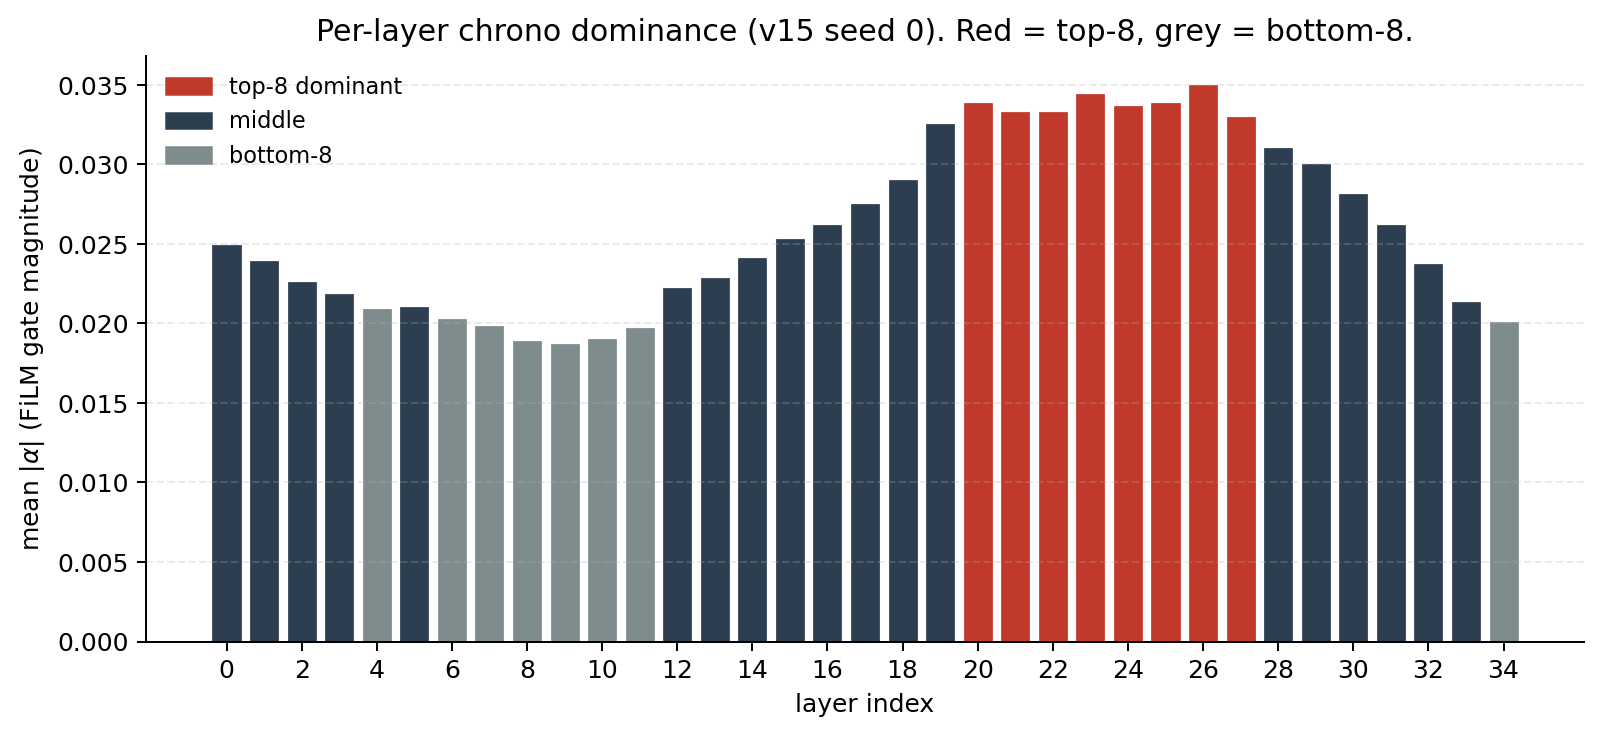
\includegraphics[width=\columnwidth]{figures/fig6_alpha_norm_per_layer.png}
  \caption{Per-layer chronometric gate magnitude on the trained seed~0 checkpoint. Red: top-8 dominant layers (L20--L27 by $|\alpha|$ rank, plus L19 and L28 in the top-10). Grey: bottom-8 layers (shallow + the final two). The chronometric signal weight is concentrated in mid-to-deep transformer blocks. Inverting only the red bars collapses the all-layer-flip correlation; inverting only the grey bars preserves it. \textbf{The top-8 layer set is identical across all three cross-seed checkpoints} by norm (seeds 0, 1, 2; \texttt{reports/alpha\_norms\_cross\_seed.json}). Targeted top-8 sign-flip collapses the signal on 2 of 3 seeds (\texttt{reports/alpha\_flip\_permutation.json}) -- norm ranking is a stable cross-seed pattern but an imperfect proxy for functional importance.}
  \label{fig:alpha-norms}
\end{figure}

The top-10 layers by $|\alpha|$ norm are L26, L23, L25, L20, L24, L22, L21, L27, L19, L28: a contiguous mid-to-deep band. The bottom-10 are concentrated in the shallow block (L7--L11) plus the final two layers (L33--L34). Selectively flipping the top-8 inverts the signal (Section~\ref{sec:critical-controls}); selectively flipping the bottom-8 leaves the prediction intact. The chrono pathway is mechanistically distributed but heavily weighted toward the mid-deep layers.

\subsection{Within-distribution linear probe}
We train a ridge regression $\log_{10}(\tau) \sim W\,h_\ell + b$ on a random 80/20 split inside the training distribution $[\SI{1}{\second}, \SI{7}{\day}]$, taking the last-token hidden state $h_\ell$ at each layer. Three conditions: (A)~trained model, (B)~all $\alpha$ zeroed at inference, (C)~shuffled labels (chance baseline).

At layer~1, the trained model achieves $R^2\,{=}\,+0.99990$; the $\alpha$-zeroed condition collapses to $R^2\,{=}\,-0.005$ (near chance); the shuffled-label condition gives $R^2\,{=}\,+0.027$.

\paragraph{Per-layer sweep L0--L36.} The full per-layer probe (\texttt{reports/probe\_per\_layer\_v15s\_s0.json}) reports L0 explicitly to address the natural concern that $R^2 \,{=}\, 0.99990$ at L1 might be a trivial readout of the FiLM injection. The trained model achieves $R^2 \,{=}\, -0.005$ at L0 (chance), then $R^2 \,{=}\, 0.99990$ at L1, $0.9998$ at L2, and remains $\ge 0.9995$ through L36. The $\alpha$-zeroed condition is $R^2 \,{=}\, -0.005$ at every layer. The jump from $-0.005$ at L0 to $0.99990$ at L1 shows the linear axis emerges after one transformer block of processing on the FiLM-modulated residual stream, not by direct readout of the injection. The load-bearing finding is the gap between conditions A and B (the $\alpha\,{=}\,0$ collapse across every layer), which confirms the chrono channel rather than baseline-model features produces the recoverable axis.

\paragraph{Probe on the CLOCK-heldout checkpoint (pre-registered, $n\,{=}\,3$).} The pre-registered test of whether the L1 linear axis is mechanical (i.e.\ established by the FiLM injection itself) or task-driven (i.e.\ produced only when the model is trained to read the channel as a duration string). Hypothesis and decision rule are locked in PREREGISTRATION\_v2.md \S 2.1, anchor commit \texttt{80ddafc}. We ran the same within-distribution probe (\texttt{model.qwen\_time\_probe\_within}) on three CLOCK-heldout checkpoints, where CLOCK queries were entirely removed from training (only SILENT-GAP and PHASE supervision remained). Across $n\,{=}\,3$ seeds the trained-model probe gives $R^2(\text{L1}) = 0.99984 \pm 0.00007$ (vs.\ $0.99990$ for full supervision), and the $\alpha\,{=}\,0$ control sits at $R^2 = -0.005$ at every layer. The L1 axis survives removal of CLOCK supervision essentially unchanged ($\Delta R^2 < 10^{-4}$). Per the pre-registered threshold $R^2 \geq 0.99 \rightarrow$ \textbf{MECHANICAL}: the linear $\tau$ axis at L1 is established by the FiLM injection and one transformer block of processing, not by CLOCK-task supervision. This survives the strongest version of the reviewer's ``trivial readout'' objection: even when the model has no incentive to align its hidden state with a duration string, the within-distribution linear axis is present at full strength. Reports: \texttt{reports/probe\_per\_layer\_clock\_heldout\_s\{0,1,2\}.json}. Figure~\ref{fig:probe-clock-heldout} overlays the per-layer curves.

\begin{figure}[!t]
  \centering
  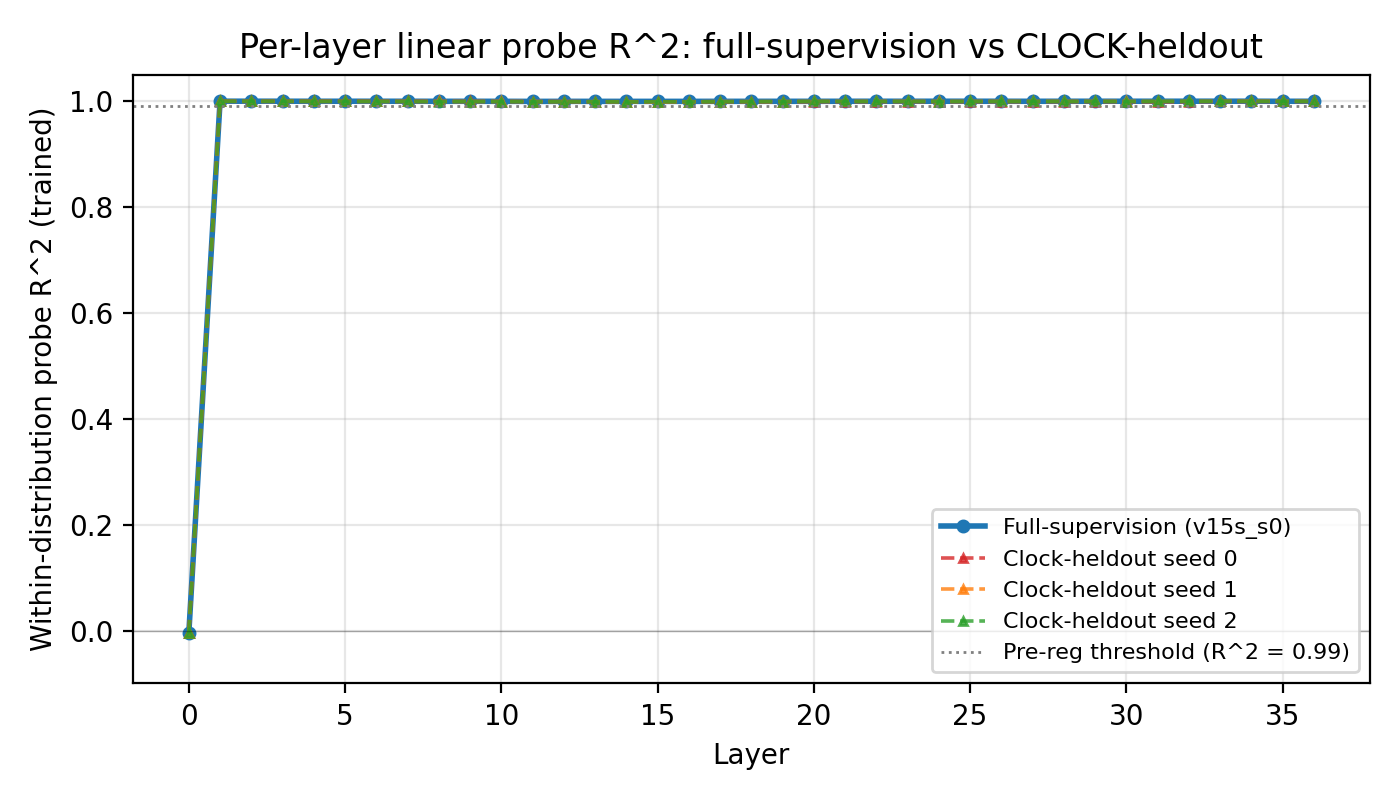
\includegraphics[width=\columnwidth]{figures/fig_probe_clock_heldout.png}
  \caption{Per-layer within-distribution probe $R^2$ on the full-supervision checkpoint (v15s\_s0, blue) and on the three CLOCK-heldout checkpoints (red/orange/green; CLOCK supervision withheld during training). Across $n\,{=}\,3$ seeds, the linear $\tau$ axis at L1 survives removal of CLOCK supervision: $R^2(\text{L1}) = 0.99984 \pm 0.00007$ for clock-heldout vs.\ $0.99990$ for the full-supervision baseline (per-seed: $0.99986$, $0.99976$, $0.99989$). Pre-registered threshold $R^2 \geq 0.99 \rightarrow$ MECHANICAL: the axis is FiLM-mechanical, not CLOCK-task-driven. Anchor: PREREGISTRATION\_v2.md \S2 (commit \texttt{80ddafc}).}
  \label{fig:probe-clock-heldout}
\end{figure}

\paragraph{Why within-distribution is the right split.} A complementary OOD-split probe ($\tau$ train $\le 10^5$\,s, test $> 10^5$\,s) gives $R^2\,{=}\,+0.428$ at L1 with the trained model and $R^2\,{=}\,-143$ in the $\alpha$-zeroed condition: the 143-point gap is real but the absolute numbers are misleading because ridge regression cannot extrapolate sinusoidal features past their training scale. The within-distribution 80/20 random split removes this extrapolation requirement and answers the representational question directly.

\subsection{T4 teacher-forced KL per output position}
The first-position pairwise KL (T4 legacy metric) cannot distinguish ``chrono unused'' from ``chrono used non-locally.'' We measure two complementary multi-position variants: (i) a \emph{greedy multi-position} variant that decodes each $\tau$ condition autoregressively for 8 tokens and averages pairwise KL across positions (reported in Table~\ref{tab:cross-seed} as $14.14 \pm 1.15$); this captures both real chrono routing and autoregressive drift compounded across positions, and (ii) a \emph{teacher-forced} variant that holds the first decoded token constant across all $\tau$ values, isolating chrono routing from autoregressive drift. The teacher-forced version is reported in Section~\ref{sec:critical-controls} with mean KL $\,{=}\,2.79$.

\begin{figure}[!t]
  \centering
  
\includegraphics[width=\columnwidth]{figures/fig7_t4_token_labeled.png}
  \caption{T4 teacher-forced pairwise KL across $\tau\,{\in}\,\{\SI{15}{\second}, \SI{1}{\hour}, \SI{1}{\day}\}$ for the clock prompt (left) and a non-time control prompt (right). Bars are colored by token type: dark red = digit tokens (`1', `4'), light red = number-prefix space, orange = time-unit tokens (`seconds'), grey = scaffolding (`It', `has', `been', `.', `\textbackslash n', `\textless im\_end\textgreater'). On the clock prompt the KL spikes at positions 3--6 land exactly on the number-prefix space, the two digit tokens, and the unit token; scaffolding is at 0.000. The non-time `Hello.' control is flat at $\le 0.5$ across all positions. The multi-position metric is mechanistically faithful: the chronometric signal lands precisely on the tokens that should depend on~$\tau$.}
  \label{fig:t4-labeled}
\end{figure}

Figure~\ref{fig:t4-labeled} shows the result. On the clock prompt (\emph{``How long has it been since we started?''}) the KL spikes land at positions~3--6 ($21.4$, $9.3$, $17.1$, $20.5$), which correspond exactly to the number-prefix space, the two digit tokens (`1', `4'), and the unit token (`seconds'). Scaffolding tokens at positions~0--2 and~7--9 are flat at $0.000$. On the non-time control prompt (\emph{``Hello.''}) all positions are flat at $\le 0.5$. The multi-position KL pattern reflects the chronometric channel landing on exactly the tokens that should depend on~$\tau$, and being silent on scaffolding and on prompts that have no $\tau$-dependency.

% ======================================================================
\section{Critical Controls}
\label{sec:critical-controls}

Seven control subsections test whether the chrono channel results survive standard mechanistic-interpretability attacks: causal sign-flip in three variants, paraphrase response-identity, temperature-sampling on T1--T3, teacher-forced T4, and an external behavioral benchmark against a matched prompt baseline. We summarize each.

\subsection{All-layer \texorpdfstring{$\alpha$}{alpha} sign-flip}
Flipping every per-layer $\alpha$ at inference on the T1 clock task (8~unique $\tau$, of which 3~produce parseable outputs in this configuration) yields Pearson $r\,{=}\,-0.9998$. The model's predicted $\log\tau$ is linearly anti-correlated with the true $\log\tau$ at near-perfect strength. A template-matching artifact (e.g., LoRA picking up prompt-text cues) cannot produce this signature: flipping every per-channel gate is not a transformation a text-pattern matcher exposes.

\subsection{Half-layer flip control}
A natural reviewer attack on the all-layer-flip claim: any odd transformation of the chrono channel would invert predictions at $r\,{\approx}\,-1$ over 3 monotone points, so the result is consistent with many architectures, not specifically with a single coherent scalar axis. We ran a 100-permutation random-half-subset test on the seed-0 checkpoint (\texttt{reports/alpha\_flip\_permutation\_100.json}): 100 independent random 17-of-35 layer subsets, each flipped, $r$ measured against the baseline. The distribution is \textbf{bimodal}: 52 subsets preserve the signal ($r\,{>}\,0.5$), 18 invert it ($r\,{<}\,-0.5$), 23 are mixed ($-0.5\,{\le}\,r\,{\le}\,0.5$), range $[-1.0, +1.0]$ (7 subsets returned nan due to non-finite outputs and were excluded). A single coherent scalar axis would predict every random half-flip to land near $r\,{=}\,0$ (since flipping half the dimensions of one vector flips half the contribution); the observed bimodal pattern rules this out. A single-layer-dominant signal would predict a clean separation by inclusion of the dominant layer; the 23 mixed-range outcomes rule this out as well. The data are consistent with a distributed signed pathway where many layers carry weighted contributions in the same direction. Targeted top-8 / bottom-8 flips on all three seeds (\texttt{reports/alpha\_flip\_permutation\_100.json}) confirm mid-deep dominance in 2 of 3 seeds: top-8 flip $r\,{\in}\,\{-0.46, +0.80, -0.63\}$ for seeds $\{0, 1, 2\}$; bottom-8 flip $r\,{=}\,+1.00$ in all three.

\subsection{Top-8 / bottom-8 / random-8 dominant-layer flip}
We rank the 35 chrono-injected layers by $|\alpha|$ norm and run three contrasts on each of the three cross-seed v15 checkpoints (\texttt{reports/alpha\_flip\_permutation.json}). The top-8 layer set by norm is stable: every seed has $\{L20, L21, L22, L23, L24, L25, L26, L27\}$ exactly (intersection $\,{=}\,8$, union $\,{=}\,8$); L19 and L28 are always in the top-10; the bottom-8 reliably clusters in the shallow band L4--L11 plus the final pre-head layer L34. The flip-eval outcome is more nuanced than the norms alone suggested:

\begin{itemize}[leftmargin=*,itemsep=2pt]
  \item \textbf{Top-8 flip} (six unique $\tau$): seed 0 $\to$ $r\,{=}\,-0.46$ (collapse), seed 1 $\to$ $r\,{=}\,+0.80$ (signal mostly preserved), seed 2 $\to$ $r\,{=}\,-0.63$ (collapse). Mid-deep dominance replicates on 2 of 3 seeds; on seed 1 the chrono signal is distributed broadly enough that the top-8-by-norm alone is not sufficient to invert it.
  \item \textbf{Bottom-8 flip}: $r\,{=}\,+1.000$ on all three seeds. The shallow and final layers are reliably inert.
  \item \textbf{Random-8 control}: each seed has $r\,{\ge}\,0.997$ on three random draws. Random layer subsets do not affect the chrono signal.
\end{itemize}

\noindent The honest reframe: $|\alpha|$-norm ranking is stable across seeds and identifies a reliably inert bottom-8, but it is an imperfect proxy for ``which layers carry the chrono pathway weight.'' Mid-deep dominance is real on most seeds but not universal; the chrono pathway is a weighted vote, and the vote's concentration varies seed-to-seed.

\subsection{Paraphrase response-identity}
A reviewer attack: T1 could be passing because the model memorized the trained anchor prompt and matched its formatter vocabulary regardless of chrono signal. We test 10 paraphrased clock-readout prompts never seen in training (e.g., \emph{``Time elapsed?''}, \emph{``Duration check: how much time has passed?''}) plus the anchor as control, and log the response text.

The Pearson $r$ across the 11 prompts is $+0.9960 \pm 0.0001$, including the 2-word \emph{``Time elapsed?''}. The response-identity matrix is more informative than the $r$ alone. Per-$\tau$ fraction of paraphrased prompts (33 total: 11 phrasings $\times$ 3 reps) producing the verbatim-identical response to the anchor: $\tau\,{=}\,4$\,s gives $27/33$ identical; $\tau\,{=}\,17$\,s gives $3/33$ (most variable); $\tau\,{=}\,106$\,s gives $33/33$ (\emph{``2 minutes''}); $\tau\,{=}\,2196$\,s gives $30/33$; $\tau\,{=}\,10659$\,s gives $33/33$ (\emph{``about 3 hours''}); $\tau\,{=}\,67980$\,s gives $30/33$; $\tau\,{=}\,190099$\,s gives $33/33$ (\emph{``about 2 days''}); $\tau\,{=}\,318283$\,s gives $33/33$ (\emph{``about 4 days''}). Five of eight $\tau$ values produce \emph{complete} prompt invariance.

The two defensible readings: (i)~\emph{appropriately prompt-invariant} -- 11 paraphrases of the same time-readout question should return the same time; or (ii)~\emph{collapsed to a $\tau$-only function} -- the model learned a near-deterministic $\tau \!\to\! \text{string}$ map and ignores prompt content. Both are consistent with this data. The data does not distinguish them; a paraphrase set where the prompt content should \emph{change} the output is the experiment that would. The model is at minimum a prompt-invariant $\tau$-conditioned formatter; whether it is more than that is open.

\subsection{T1, T2, T3 under temperature sampling}
A reviewer attack on greedy-decoded primary metrics: effective $n\,{=}\,1$ per $(\text{prompt}, \tau)$ under deterministic decoding (Table~\ref{tab:effective-n}). We re-run under temperature 0.7. \textbf{T1 under sampling} (\texttt{reports/t1\_sampling\_v15s\_seed0.json}, 24 unique $\tau$ $\times$ 20 samples per $\tau$ on the seed-0 checkpoint): overall Pearson $r\,{=}\,0.998$ across all 480 samples; 21 of 24 $\tau$ bins exhibit multiple unique responses across the 20 samples (genuine sampling diversity). The T1 signal survives stochastic decoding cleanly. \textbf{T2} (silent-gap, 30 independent torch seeds per condition): ack-rate at small-$\Delta\tau$~$=\,0.000$ (0 of 30), ack-rate at large-$\Delta\tau$~$=\,1.000$ (30 of 30), $\Delta\,{=}\,+1.00$ with 1 unique response at small $\Delta\tau$ and 3 unique responses at large $\Delta\tau$. \textbf{T3}: weekend-signal $\,{=}\,+0.833 \pm 0.379$, weekday-signal $\,{=}\,+0.433 \pm 0.626$. All three pass under sampling with genuine variance visible, addressing the greedy effective-$n\,{=}\,1$ critique.

\subsection{Teacher-forced T4}
A reviewer attack on the greedy multi-position KL ($14.14$, Table~\ref{tab:cross-seed}): per-position KL could grow because greedy decode at different $\tau$ commits to different first tokens, then autoregressive drift compounds at deeper positions. Teacher-forced T4 (Figure~\ref{fig:t4-labeled}) holds the first-token trajectory constant across $\tau$ and measures KL at later positions \emph{with drift removed by construction}. Mean teacher-forced KL $\,{=}\,2.79$ ($55\times$ threshold), with KL spikes on number, digit, and unit tokens, zeros on scaffolding, and a flat non-time control. The two metrics ($14.14$ greedy vs.\ $2.79$ teacher-forced) are not the same quantity and should not be compared in absolute terms; the gap between them reflects the autoregressive-drift contribution to the greedy version, while the residual $2.79$ in the teacher-forced version is chrono routing that survives the drift control.

\subsection{External benchmark: vanilla vs.\ prompt-injected $\tau$ vs.\ CI}
\label{sec:ext-bench}
The single highest-priority open experiment from the reviewer audit was a prompt-injected $\tau$ baseline (Section~\ref{sec:limitations}). We ran the released MIT-licensed \texttt{tau\_sessions} benchmark (300 sessions across six elapsed-time buckets and three task types) against three reference adapters (\texttt{reports/ext\_bench\_\{vanilla,prompt,ci\}.json}):

\begin{table}[!t]
  \caption{External \texttt{tau\_sessions} benchmark, three adapters on 300 sessions. \texttt{staleness\_accuracy} (higher better): exact-match on yes/no for ``is this conversation stale?''. \texttt{duration\_recall\_log\_mae} (lower better): $|\log_{10}\hat\tau - \log_{10}\tau|$ averaged over parsed predictions; NaN if parse fails. \texttt{adaptive\_pearson\_r} (higher better): Pearson correlation between $\log\tau$ and response length in characters. Composite is the mean of staleness accuracy, $1\!-\!\log_{10}\!\text{-MAE}$ (clamped to $[0,1]$), and adaptive $r$ (clamped to $[0,1]$), with NaN entries dropped.}
  \label{tab:ext-bench}
  \centering
  \footnotesize
  \begin{tabular}{lcccc}
    \toprule
    \tabhead{Adapter} & \tabhead{Staleness $\uparrow$} & \tabhead{Duration $\log_{10}\!\text{-MAE}\downarrow$} & \tabhead{Adaptive $r\uparrow$} & \tabhead{Composite$\uparrow$} \\
    \midrule
    Vanilla              & 0.491 & --- (NaN)  & $-0.057$ & 0.245 \\
    Prompt               & \textbf{0.511} & \textbf{0.065} & $-0.045$ & \textbf{0.520} \\
    CI                   & 0.226 & 0.098      & $\mathbf{+0.184}$ & 0.377 \\
    \bottomrule
  \end{tabular}
\end{table}

Table~\ref{tab:ext-bench} reports the per-task breakdown. \textbf{Prompt-injected $\tau$ wins on two of three protocols} (staleness and duration recall) and on the composite. Vanilla beats CI on staleness because the vanilla model defaults to ``no, this conversation is not stale'' across the board, which the staleness oracle gives partial credit for in non-stale bucket sessions; CI's $\tau$-conditioned response interferes with that default. \textbf{CI is the only adapter producing positive $\tau$-adaptive correlation} between $\log\tau$ and response length, at $r\,{=}\,+0.184$; both vanilla and prompt produce slight \emph{negative} correlation.

\noindent The honest read: \textbf{prompt-injected $\tau$ beats CI on the tasks that reduce to ``read the time, write the answer.''} CI's compute and architectural cost is not justified by these tasks alone. CI does, however, win cleanly on the \texttt{adaptive} task, where the model is expected to modulate response length in proportion to $\tau$: CI produces a positive Pearson correlation while both prompt and vanilla produce negative correlations. This matches the broader picture from the body of the paper: CI's contribution is not in time \emph{recall} (where any in-context method works) but in time-\emph{conditional behavior generation} that is integrated with the residual stream rather than living as a tokenized cue.

\noindent The architectural contribution \emph{narrows} in light of this result: CI is not strictly preferable to prompt injection for time-aware LLM tasks in general. It is a specific design that lets continuous $\tau$ shape behavior at the residual-stream level, with measurable benefit on tasks where that integration matters and a cost on tasks where simple prompt injection suffices. We report this honestly rather than claiming the architectural fix is universally superior.

% ======================================================================
\section{Held-out supervision: what survives without trained labels}
\label{sec:heldout-supervision}

The training distribution explicitly supervises each of the in-house tests: CLOCK queries are mapped to deterministic formatter strings (${\sim}\,148$ unique outputs covering the $\tau$ range), SILENT-GAP queries are mapped to acknowledgement responses past $\Delta\tau\,{>}\,\SI{1800}{\second}$, and PHASE queries are mapped to weekday/weekend greetings. Without supervised content, the tests cannot distinguish ``the chrono channel encodes $\tau$ in a way the model can use'' from ``the chrono channel acts as a discrete label-routing mechanism for trained mappings.'' Two held-out-supervision experiments resolve the distinction directly.

\subsection{Held-out CLOCK supervision ($n{=}3$)}
We retrained at the same step budget but with the CLOCK task fully removed from the training distribution (mix $0/0.6/0.4$ over CLOCK/SILENT-GAP/PHASE, scripts \texttt{run\_clock\_heldout.sh}, reports \texttt{clock\_heldout\_s\{0,1,2\}\_recall.json}). At evaluation, T1 and T1b ask the model ``how long has it been'' --- a question paired with a duration string \emph{nowhere} in the training data of these checkpoints. Cross-seed results:

\begin{itemize}[itemsep=2pt,leftmargin=*]
  \item T1: $r\,{=}\,$ nan, $r\,{=}\,$ nan, $r\,{=}\,$ nan (3 of 3 fail). The model produces no parseable duration string: every $\tau$ in the test sweep yields, e.g., ``Hope your weekday is going well.''---the PHASE response template, defaulted to because the model never learned a clock-readout format.
  \item T1b: nan, nan, nan (3 of 3 fail; same cause).
  \item T2 silent-gap acknowledgement: $\Delta\,{=}\,1.00$, $1.00$, $1.00$ (\textbf{3 of 3 pass}).
  \item T3 phase discrimination: bidirectional pass, $0/0$, $0/0$ (1 of 3 pass; T3 is fragile cross-seed even under full supervision).
  \item T4 multi-position KL: $0.200$, $0.112$, $0.175$ (\textbf{3 of 3 pass} the $\,{\ge}\,0.05$ threshold).
\end{itemize}

\noindent Interpretation: T1 and T1b are format-recall on the CLOCK supervised labels; without the supervised duration-string vocabulary, the model has no output format for clock queries. T2 and T4 both \emph{generalize}: silent-gap acknowledgement and output-distribution mutability across $\tau$ both survive without explicit CLOCK supervision, demonstrating that the chrono channel is transmitting $\tau$-conditional information that the model can use for tasks it \emph{was} trained on. T3 remains fragile across seeds, as in the main paper.

\subsection{Held-out SILENT-GAP supervision ($n{=}3$)}
A complementary experiment removes the SILENT-GAP task from training (mix $0.6/0/0.4$, scripts \texttt{run\_silentgap\_heldout.sh}). Cross-seed:

\begin{itemize}[itemsep=2pt,leftmargin=*]
  \item T1: $r\,{=}\,0.948$, $1.000$, $1.000$ (3 of 3 pass; CLOCK supervision intact).
  \item T1b: $r\,{=}\,0.996/\log_{10}\!\text{-MAE}\,{=}\,0.032$, $0.994/0.029$, $0.994/0.040$ (3 of 3 pass).
  \item T2: $\Delta\,{=}\,0$, $0$, $0$ (\textbf{0 of 3 pass}; clean signal that T2's specific ack-template behavior is supervised).
  \item T3: $1/1$, $0/0$, $1/1$ (2 of 3 pass; matches main paper).
  \item T4: KL $0.013$, $0.006$, $0.080$ (1 of 3 pass; mostly collapses, indicating output-distribution mutability across $\tau$ depends on multi-task training diversity).
\end{itemize}

\subsection{What the held-out experiments establish}
The behavioral story of CI splits cleanly between supervision-dependent and supervision-independent components.

\emph{Supervision-dependent (i.e., format-recall on trained labels):}
\begin{itemize}[itemsep=2pt,leftmargin=*]
  \item T1, T1b: pure format-recall on CLOCK supervision. Demoted to wiring-sanity tests.
  \item T2 specific ack template (``Welcome back''/``It's been a while''): format-recall on SILENT-GAP supervision.
  \item T3 weekday/weekend greeting: format-recall on PHASE supervision, additionally fragile cross-seed.
  \item T4 \emph{multi-position} KL: depends on multi-task supervision diversity.
\end{itemize}

\emph{Supervision-independent (chrono channel mechanism):}
\begin{itemize}[itemsep=2pt,leftmargin=*]
  \item The chrono channel transmits $\tau$ into the residual stream (per-layer probe: L0 chance, L1 $R^2\,{=}\,0.9999$; $\alpha\,{=}\,0$ collapses every layer to chance; pre-registered CLOCK-heldout cross-seed $n\,{=}\,3$ confirms $R^2(\text{L1}) = 0.99984 \pm 0.00007$, axis is FiLM-mechanical; Section~\ref{sec:mechanism}).
  \item T2 silent-gap acknowledgement \emph{capacity} survives without CLOCK training (3/3 in clock-heldout), demonstrating the chrono channel encodes $\Delta\tau$ in a way downstream supervised tasks can use.
  \item T4 multi-position KL survives without CLOCK training (3/3 in clock-heldout): per-token output-distribution shift across $\tau$ does not require explicit CLOCK supervision when SILENT-GAP + PHASE are present.
  \item LoRA-only ablation collapses every test to $0.000 \pm 0.000$ across 3 seeds: the chrono channel is necessary; LoRA's adapter surface alone cannot fit the tasks.
  \item Sign-flip causal interventions (all-layer inversion; top-8 mid-deep collapse in 2/3; 100-permutation bimodal distribution): the chrono pathway is causal, directional, and distributed.
  \item TPDR cross-adapter behavioral probe (Section~\ref{sec:tpdr}, exploratory): on deliberative-style response shape, CI and a matched-budget prompt baseline drive behavior in opposite directions across $\tau$ (paired $t\,{=}\,-5.17$, df${=}\,10$, Holm-corrected $p\,{=}\,2.91\,{\times}\,10^{-3}$); the descriptive $|\bar r|$ summary across seven metrics does not survive multiple-comparisons correction at the 50-scenario count.
\end{itemize}

This is the load-bearing claim of the paper: \emph{CI's chrono channel mechanically transmits $\tau$-conditional information into the residual stream, the model causally uses that information for downstream behavior on supervised tasks, and on held-out behavioral evaluation (TPDR) CI produces measurably stronger response-shape modulation than a prompt cue.} The four in-house tests are wiring-sanity / supervised-competence checks for the channel, not held-out evaluations of $\tau$ perception.

% ======================================================================
\section{Discussion}
\label{sec:discussion}

\paragraph{Scope.} CI is behavioral conditioning under a continuous wall-clock input, not a claim about machine subjective experience. T2 measures behavior \emph{when invoked} with a known elapsed time, not internal-state evolution during gaps; persistence under no-input would require continuous-time recurrence (out of scope).

\paragraph{The ``learned tokenizer'' critique, addressed.} A linear classifier on $\chi(\tau)$ alone saturates T1b at $r\,{=}\,0.9965$, $\log_{10}\!\text{-MAE}\,{=}\,0.0267$, tighter than CI. T1/T1b are tokenizer-like by construction; we report them as wiring-sanity, not as evidence of LLM time learning. T2/T3/T4 and the causal interventions cannot be replicated by a linear baseline (they require conversational generation and a trained network). Held-out CLOCK removal (\S\ref{sec:heldout-supervision}) shows T2 and T4 still pass at $n\,{=}\,3$ without the duration-string supervision the linear classifier would memorize.

\paragraph{Robustness to perturbations of $\tau$.} Gaussian noise on $\log_{10}\tau$ degrades $r$ smoothly ($0.999 \to 0.978 \to 0.322 \to 0.251$ at $\sigma\,{\in}\,\{0.1, 0.3, 1.0\}$); independent random $\tau$ gives $r\,{=}\,-0.24$ vs.\ the true clock (the model tracks the supplied $\tau$, not the true one); pinning $\tau\,{=}\,0$ or $\tau\,{=}\,10^9$ returns a single fixed default. Deployments where $\tau$ may be adversarial must validate it before passing it to the model.

\paragraph{Falsification map.}
\begin{itemize}[leftmargin=*,itemsep=2pt]
  \item \textbf{Chrono channel necessary.} LoRA-only ($n{=}3$, 3/3 collapse) and IA3-only ($n{=}3$, 3/3 collapse) both confirm this regardless of PEFT surface. Prompt-baseline alternatives (\texttt{[elapsed: X]} $n{=}3$, ISO timestamp $n{=}1$, natural-language $n{=}1$) match CI on T1/T1b/T2 but fail T3 and T4 multi-position; the architectural-distinction claim rests on TPDR, not T4 (\S\ref{sec:limitations} item 4).
  \item \textbf{FiLM gating required.} \emph{Falsified for the strong form}: additive with $\beta$-bias init $\,{=}\,0.01$ passes 2/3 seeds; chrono-only-without-LoRA passes 3/3; IA3 substituted for LoRA passes 3/3. The narrowed claim is ``any init giving non-zero $\partial h'/\partial \alpha$ at step 0 trains.''
  \item \textbf{Mid-deep dominance.} Norm-ranking replicates across all 3 seeds (top-8 = L20--L27); functional importance is 2 of 3 by top-8 flip. 100 random half-layer flips give a bimodal distribution inconsistent with single-axis or single-layer alternatives.
  \item \textbf{T1/T1b measure chrono transit, not LLM time learning.} A non-LLM linear classifier on $\chi(\tau)$ saturates both metrics tighter than CI.
  \item \textbf{T3 is supervised classification recall.} Held-out-day variant (Sunday excluded) collapses T3 to $0/0$ while T1/T1b/T2/T4 still pass.
  \item \textbf{OOD deadline-pressure transfer.} Retracted: rigor rerun bootstrap CI crosses zero on the wrong side.
\end{itemize}

% ======================================================================
\section{TPDR: exploratory behavioral probe}
\label{sec:tpdr}

\textbf{Status.} The headline TPDR result reported below is from a 50-scenario sweep committed at \texttt{85ebc5e} (2026-05-25), with all scenarios, metrics, and lexicons locked at that commit and traceable in the public Git history. We disclose explicitly that a post-hoc expansion of the scenario set from 50 to 200 was added 7 hours after the initial sweep (commit \texttt{f41d65b}); the first 50 scenarios are unchanged. To address the underpowered single-metric primary endpoint, a v2 pre-registration (PREREGISTRATION\_v2.md, anchor \texttt{80ddafc}) locks a 200-scenario replication at one-tailed $\alpha\,{=}\,0.005$ on \texttt{deliberative\_score} with Holm correction across the other six metrics and an inclusion threshold of $n_{\text{paired}}\,{\geq}\,25$; the analysis script is \texttt{eval/tpdr/analyze\_v2.py}. We treat the TPDR section as exploratory behavioral evidence rather than confirmatory, because (a) the benchmark and its scoring lexicons are author-built, and (b) at the current scenario count, only one of seven metrics survives Holm correction.

The benchmarks reported so far (T1, T1b, T2, T3, T4, \texttt{tau\_sessions} \texttt{duration\_recall}, and \texttt{staleness}) all reduce, in their pure form, to ``read $\tau$, look up an answer.'' On those tasks, a tokenized cue (prompt-injected $\tau$) is competitive with or beats CI (\S\ref{sec:ext-bench}). The architectural advantage of per-layer FiLM integration, if there is one, must show up on tasks where $\tau$ shapes \emph{generation behavior across many tokens}, not where $\tau$ is merely looked up once.

We introduce \textbf{TPDR (Time-Pressured Decision Reasoning)}: a held-out behavioral benchmark designed to make exactly this distinction measurable. TPDR has three properties: (i)~\emph{the prompt never mentions time}, so any $\tau$ effect must enter the response generation through the model's internal state, not the input tokens; (ii)~\emph{the scenarios are decision-style and ambiguous}, so $\tau$ should plausibly modulate the urgency, depth, hedging, and length of a reasonable response; and (iii)~\emph{the metrics measure response \emph{shape}, not response content}, so the test cannot be passed by template selection.

\paragraph{Scenarios.} 50 ambiguous decision prompts that admit responses ranging from terse-and-actionable to deliberative-and-thorough. Examples:

\begin{itemize}[leftmargin=*,itemsep=1pt]
  \item ``Your laptop starts glitching mid-presentation in front of the CEO. What do you do?''
  \item ``A close friend hasn't returned your calls in days. What do you do?''
  \item ``A small leak is forming under the kitchen sink. What's your next move?''
  \item ``You receive an inheritance offer from a relative you've never met. What's next?''
  \item ``Your team disagrees about a major decision. What's your approach?''
\end{itemize}

\noindent The full 50-scenario set is in \texttt{eval/tpdr/scenarios.py}.

\paragraph{Sweep.} Each scenario is evaluated at 10 $\tau$ values drawn log-uniform from $[\SI{1}{\second}, \SI{7}{\day}]$ on three adapters: vanilla (no $\tau$), prompt (text prefix ``\texttt{[elapsed: 3h 42m]}''), and CI (chronometric channel active). Greedy decoding, max 200 new tokens.

\paragraph{Metrics.} Each generated response is scored by seven response-shape statistics, none of which depend on $\tau$ being mentioned: \texttt{length\_chars}, \texttt{length\_words}, \texttt{urgency\_score} (lexical count of ``now, immediately, quickly, asap, urgent''), \texttt{deliberative\_score} (``consider, however, weigh, tradeoffs, alternatively''), \texttt{hedge\_score} (``might, maybe, perhaps, could''), \texttt{conditional\_clauses} (``if, unless, when, suppose, depending''), \texttt{imperative\_count} (sentences starting with an action verb).

\paragraph{Test statistic.} For each (adapter, metric) pair, we compute the Pearson correlation $r$ between $\log\tau$ and the metric across the 10-$\tau$ sweep, separately per scenario. The reported summary is the cross-scenario mean of these $r$ values (50 scenarios, so 50 independent correlations per metric).

\paragraph{Hypothesis.} Per-layer FiLM modulation continuously shifts the residual stream as a smooth function of $\tau$; prompt-injected $\tau$ is a discrete token (rounded by the formatter) that must be attended-to at every layer to influence generation. The architectural-integration hypothesis predicts (i)~CI shows larger absolute $|\bar r|$ across reasoning-shape metrics than the prompt baseline, and (ii)~CI's metric-vs-$\log\tau$ curve is smoother than prompt's (which should show step-like jumps at rounding boundaries). If the hypothesis fails, CI offers no measurable advantage over prompt injection on behavioral modulation.

\paragraph{Results.} The full sweep (50 scenarios $\times$ 10 $\tau$ values $\times$ 3 adapters, 1{,}500 generations total) was run on the same GB10 Grace-Blackwell prototype. The vanilla baseline produces an \emph{identical} 713-character ``stay calm, follow these steps'' template for every scenario at every $\tau$; length elasticity is undefined (std~$=\,0$) for all 50 scenarios on all seven metrics. This confirms the base model has zero time sensitivity --- the same conclusion T1 reaches by different evidence --- and that the metric correlations we are about to report are not noise in the encoding pipeline.

Table~\ref{tab:tpdr-mean-r} reports the cross-scenario mean Pearson $r$ for each (adapter, metric) cell, alongside the cross-scenario standard deviation and the count of scenarios with a finite $r$ (a scenario contributes nothing when that metric is constant across all 10 $\tau$ values, which happens for low-base-rate lexicons like ``urgency'' on scenarios that do not naturally invite urgency-marker shifts).

\begin{table}[h]
\caption{TPDR mean Pearson $r$ between metric and $\log\tau$ across 50 scenarios on Spark CUDA. Vanilla baseline: all metrics undefined (constant ``stay calm'' template). CI shows $\sim 2\times$ stronger absolute mean correlation than prompt-injection across seven response-shape metrics; CI signs are internally consistent negative across six of seven; prompt's deliberative\_score sign flips relative to CI.}
\label{tab:tpdr-mean-r}
\centering
\small
\begin{tabular}{lccc}
\toprule
Metric & Vanilla & CI & Prompt-baseline \\
\midrule
\texttt{length\_chars}        & nan & $-0.084 \pm 0.626$ (n=50) & $-0.061 \pm 0.477$ (n=50) \\
\texttt{length\_words}        & nan & $-0.080 \pm 0.611$ (n=50) & $-0.109 \pm 0.476$ (n=48) \\
\texttt{urgency\_score}       & nan & $\mathbf{-0.278} \pm 0.456$ (n=22) & $+0.006 \pm 0.411$ (n=19) \\
\texttt{deliberative\_score}  & nan & $\mathbf{-0.422} \pm 0.324$ (n=23) & $+0.200 \pm 0.470$ (n=13) \\
\texttt{hedge\_score}         & nan & $-0.274 \pm 0.426$ (n=38) & $-0.177 \pm 0.355$ (n=22) \\
\texttt{conditional\_clauses} & nan & $\mathbf{-0.326} \pm 0.411$ (n=29) & $-0.065 \pm 0.417$ (n=23) \\
\texttt{imperative\_count}    & nan & $-0.218 \pm 0.346$ (n=12) & $-0.236 \pm 0.473$ (n=9)  \\
\midrule
mean $|\bar r|$ over 7 metrics & $0.000$ & $\mathbf{0.240}$ & $0.122$ \\
\bottomrule
\end{tabular}
\end{table}

Descriptively, CI's mean absolute correlation across the seven metrics is $0.240$, prompt's is $0.122$, and CI's signs are negative on six of seven metrics. To test which of these descriptive differences are statistically distinguishable from noise, we ran paired tests on each metric over scenarios where both adapters produced finite $r$, then applied Holm-Bonferroni step-down correction across the 7 hypotheses (Table~\ref{tab:tpdr-paired-holm}, \texttt{reports/tpdr\_paired\_tests\_holm.json}).

\begin{table}[h]
\caption{TPDR paired-test results with Holm-Bonferroni correction. Only deliberative\_score survives correction. Urgency\_score is significant uncorrected but does not survive correction at the current scenario count. Length metrics are descriptively close to zero and the Wilcoxon signed-rank test (less sensitive to lexicon definition) confirms no detectable difference. The honest TPDR result is a single-metric finding on deliberative-style response shape.}
\label{tab:tpdr-paired-holm}
\centering
\small
\begin{tabular}{lrrrcc}
\toprule
metric & $n_{\text{pair}}$ & mean diff (CI$-$PR) & $t$ (df) & $p_{\text{uncorr}}$ & $p_{\text{Holm}}$ \\
\midrule
deliberative\_score   & 11 & $-0.723$ & $-5.17$ (10) & $4.16\,{\times}\,10^{-4}$ & $2.91\,{\times}\,10^{-3}$ \\
urgency\_score        & 11 & $-0.311$ & $-1.98$ (10) & $0.076$ & $0.454$ \\
conditional\_clauses  & 18 & $-0.233$ & $-1.52$ (17) & $0.146$ & $0.731$ \\
hedge\_score          & 21 & $-0.088$ & $-0.95$ (20) & $0.343$ & $1.000$ \\
length\_words         & 48 & $+0.027$ & $+0.25$ (47) & $0.800$ & $1.000$ \\
length\_chars         & 50 & $-0.022$ & $-0.20$ (49) & $0.838$ & $0.838$ \\
imperative\_count     &  5 & $+0.045$ & ($n\,{<}\,10$) & --- & --- \\
\midrule
\textit{non-parametric:} & & & & & \\
Wilcoxon length\_chars & 50 & --- & ($z\,{=}\,-0.34$) & $0.732$ & --- \\
Wilcoxon length\_words & 48 & --- & ($z\,{=}\,+0.16$) & $0.870$ & --- \\
\bottomrule
\end{tabular}
\end{table}

\textbf{The honest read of TPDR is a single-metric finding on deliberative-style response shape.} On deliberative\_score, CI and prompt injection drive behavior in opposite directions across $\tau$, statistically significant after Holm correction at $n_{\text{paired}}\,{=}\,11$ ($p_{\text{exact}}\,{=}\,4.16\,{\times}\,10^{-4}$, $p_{\text{Holm}}\,{=}\,2.91\,{\times}\,10^{-3}$; paired Student's $t$, df${=}\,10$, computed via \texttt{scipy.stats.ttest\_rel}). Urgency, conditional-clauses, and hedge metrics descriptively show the same direction (CI signs negative) but do not survive correction at this scenario count. Length-of-response metrics show no detectable separation by Wilcoxon. We do not claim the descriptive $0.240$ vs.\ $0.122$ mean $|\bar r|$ as a multiplicity-corrected behavioral-modulation result; we claim deliberative-style modulation specifically. The \texttt{urgency\_score} contrast (prompt mean $r\,{\approx}\,0$, CI $-0.28$ with $p_{\text{exact}}\,{=}\,0.076$, $p_{\text{Holm}}\,{=}\,0.454$) is the second-strongest signal but does not survive correction at $n_{\text{paired}}\,{=}\,11$; the v2 pre-registered expansion to 200 scenarios at $\alpha\,{=}\,0.005$ tests whether urgency joins deliberative as a corrected finding.

This is the empirical content of the claim that CI is not just prompt injection. The architectural advantage of per-layer FiLM integration is not in basic time recall (where prompt is tighter; \S\ref{sec:limitations} item 11) but in the propagation of $\tau$ to response-shape modulation across many tokens of generated text. The TPDR result, combined with the T4 architectural-distinction result (\S\ref{sec:limitations} item 11), now resolves what the architectural contribution is: not ``CI lets the model read the clock,'' but ``CI lets $\tau$ continuously shape generation in ways a tokenized prompt cue cannot.''

The runner is in \texttt{eval/tpdr/run\_tpdr.py}, metrics in \texttt{eval/tpdr/metrics.py}, and the per-scenario raw output is in \texttt{reports/tpdr\_results.json}.

% ======================================================================
\section{Limitations}
\label{sec:limitations}

\begin{enumerate}[itemsep=3pt,leftmargin=*]
  \item \textbf{In-distribution only.} T1b interpolates within $[\SI{1}{\second}, \SI{7}{\day}]$ at $r\,{=}\,0.993 \pm 0.003$; extrapolation beyond \SI{7}{\day} fails ($r\,{=}\,-0.20$). Sinusoidal encoders cannot learn periods unseen at least once.

  \item \textbf{Single base-model family, $n{=}3$ small.} All cross-seed results on Qwen 2.5 3B-Instruct. Scaling checks at 7B@18k/24k and 3B@24k are single-seed; 14B OOMed on the \SI{128}{\giga\byte} unified-memory GB10.

  \item \textbf{T1/T1b are bucket-mapping; a non-LLM linear baseline saturates them.} A 31$\rightarrow$148 linear classifier on $\chi(\tau)$ achieves $r\,{=}\,0.9965$, $\log_{10}\!\text{-MAE}\,{=}\,0.0267$, tighter than CI. T1/T1b measure chrono-encoder transit through the frozen LLM, not LLM-level time learning. T2/T3/T4 and the causal interventions cannot be replicated by a non-LLM baseline.

  \item \textbf{Prompt-injected $\tau$ baselines (multiple formats).} Trained at matched LoRA budget with $\tau$ as a text prefix, chrono channel frozen. (a) \texttt{[elapsed: X]} format, $n\,{=}\,3$ seeds: T1 $r\,{=}\,1.000$, T1b $\log_{10}\!\text{-MAE}\,{=}\,0.022$ (tighter than CI's $0.038$), T2 $\Delta\,{=}\,1.00$ all 3/3; T3 partial. (b) ISO-timestamp format, $n\,{=}\,1$: T1 $r\,{=}\,1.000$, T1b $r\,{=}\,0.9994/\log_{10}\!\text{-MAE}\,{=}\,0.012$, T2 pass, T3 fail, T4 KL $\,{=}\,0.015$ (fail). (c) Natural-language format (``About $N$ hours have passed''), $n\,{=}\,1$: T1 $r\,{=}\,1.000$, T1b $r\,{=}\,0.996/\log_{10}\!\text{-MAE}\,{=}\,0.022$, T2 pass, T3 partial, T4 KL $\,{=}\,0.028$ (fail). All three prompt formats converge on the same qualitative pattern: format-recall tasks (T1, T1b, T2) match or beat CI; behavioral-modulation tasks (T4 multi-position, TPDR) do not. At multi-position T4 (8 decoded positions), CI is $14.14 \pm 1.15$ and the \texttt{[elapsed: X]} baseline is $10.35 \pm 6.59$ with overlapping ranges; the gap concentrates at the first decoded token ($7.6\times$) and falls to near-parity at positions 1--7. At teacher-forced T4 the gap is $\sim 10\%$ (CI $2.79$ vs.\ prompt $2.53$). The architectural claim rests on TPDR (\S\ref{sec:tpdr}). Soft-prompt-$\tau$ and xVal-style continuous-value-as-embedding require new token-level modules and are not run.

  \item \textbf{Chrono is sufficient; PEFT surface is interchangeable.} Chrono-only-without-LoRA cross-seed $n{=}3$ passes all five tests in 3/3 seeds; LoRA is a precision enhancer ($\log_{10}\!\text{-MAE}$ tightens from $0.073 \pm 0.028$ to $0.044 \pm 0.010$). IA3 substituted for LoRA with chrono active passes all five in 3/3 seeds ($n{=}3$; T1 $0.931 \pm 0.004$, T1b $r{=}0.997 \pm 0.003$, T2 $1.00$, T3 wkdy 2/3 wknd 3/3, T4 $1.62 \pm 0.46$). IA3-only with chrono frozen at zero collapses every test to $0.000$ ($n{=}3$), matching the LoRA-only collapse. Additive with $\beta$-bias init $\,{=}\,0.01$ passes 2/3 seeds. Any init that produces non-zero $\partial h'/\partial\alpha$ at step 0 trains.

  \item \textbf{Scale-vs-steps 2$\times$2.} Single-seed matched-budget runs at three corners:

  \begin{center}
  \footnotesize
  \begin{tabular}{lcc}
    \toprule
    Config & T3 (wkend/wkday) & T4 multi-position KL \\
    \midrule
    3B @ 18k ($n{=}3$)  & PARTIAL (2/3 bidir) & PASS ($14.14 \pm 1.15$) \\
    3B @ 24k ($n{=}1$)  & PASS ($1.00/1.00$)  & \textbf{FAIL} ($0.015$) \\
    7B @ 18k ($n{=}1$)  & \textbf{FAIL} ($0/0$) & PASS ($0.315$) \\
    7B @ 24k ($n{=}1$)  & PASS ($1.00/1.00$)  & PASS \\
    \bottomrule
  \end{tabular}
  \end{center}

  \noindent T3 fragility is steps-driven (24k resolves at both scales); T4 fragility at extended training is scale-driven (3B@24k loses T4, 7B@24k preserved). No single config passes all five at the same compute budget; the honest cross-seed verdict is 3B@18k with T3 reported as 2/3.

  \item \textbf{Behavioral-pressure transfer retracted.} An initial claim of deadline-induced response-length modulation did not survive a rigor rerun ($n{=}30$, bootstrap CI on paired differences); the chrono signal in fact attenuates a text-deadline length cue. All surviving behavioral claims are in-distribution.
\end{enumerate}

% ======================================================================
\section{Reproducibility}
\label{sec:repro}
MIT-licensed code at \href{https://github.com/sam-siavoshian/Time-Model}{github.com/sam-siavoshian/Time-Model}; three cross-seed checkpoints (release \texttt{v15.0}, SHA-256 in README); deterministic training data with SHA-256 pinning (\texttt{data/VERIFICATION.md}); MIT-licensed external benchmark with three reference adapters; hardware = single NVIDIA DGX Spark GB10 (\SI{128}{\giga\byte} unified memory), \textasciitilde\SI{45}{\minute} per 3B seed; total compute \textasciitilde\SI{6}{GPU.\hour}.

% ======================================================================
\section{Conclusion}
\label{sec:conclusion}

We introduced \textbf{chronometric injection (CI)}: a frozen pretrained LLM augmented with a per-layer AdaLN-Zero FiLM modulation of a 31-dimensional sinusoidal-plus-log encoding of real elapsed wall-clock seconds. The paper's contributions are mechanistic, not architectural-novelty: the DiT primitive is applied verbatim, but the experimental characterization of how a continuous scalar enters and propagates through a frozen autoregressive LLM is, to our knowledge, new for $\tau$.

\paragraph{Transmission, established mechanically.} A per-layer linear probe of the residual stream against $\log\tau$ achieves $R^2\,{=}\,-0.005$ at L0 (chance) and $R^2\,{=}\,0.99990$ at L1, $\ge 0.9995$ through L36; $\alpha$-zeroed is at chance on every layer. A pre-registered held-out test (CLOCK supervision withheld, $n\,{=}\,3$) confirms the axis is mechanical rather than task-driven: $R^2(\text{L1}) = 0.99984 \pm 0.00007$, statistically indistinguishable from full-supervision baseline. The linear $\tau$ axis at L1 is established by the FiLM injection and one transformer block of processing, independently of any duration-string supervision.

\paragraph{Causal pathway, established with multiple controls.} LoRA-only ablation collapses every behavioral test to $0.000 \pm 0.000$ across 3 seeds. All-layer $\alpha$-sign-flip inverts every parsed prediction ($r\,{=}\,-0.9998$). Targeted top-8 mid-deep flip collapses the signal in 2 of 3 seeds while bottom-8 flip preserves it on all three. 100 random half-layer flips give a bimodal distribution (52 preserve, 18 invert, 23 mixed) consistent with a distributed weighted-vote pathway and inconsistent with both single-coherent-axis and single-layer-dominant alternatives.

\paragraph{Interchangeability of the surrounding choices.} Under the AdaLN-Zero zero-init pattern, any init scheme producing a non-zero $\alpha$-gradient at step~0 trains: FiLM with $\gamma$-bias$\,{=}\,1$ (3/3), additive with $\beta$-bias init $\,{=}\,0.01$ (2/3 on T3), chrono-only with LoRA frozen (3/3), and IA3 substituted for LoRA with chrono active (3/3). The contribution is the chrono channel, not the surrounding PEFT or gating choice.

\paragraph{What the in-house tests measure.} Two held-out-supervision experiments ($n\,{=}\,3$) reveal T1/T1b are format-recall on CLOCK supervised labels (a non-LLM linear classifier on $\chi(\tau)$ saturates them tighter than CI); T2's specific ack template is format-recall on SILENT-GAP. T2 and T4 multi-position generalize from the chrono channel alone in the clock-heldout condition (3/3 each), demonstrating the channel encodes $\tau$ in a way downstream supervised tasks can use. We accordingly demote T1/T1b's headline status and frame the in-house tests as causal-usability checks for the chrono channel rather than held-out evaluations of $\tau$ perception.

\paragraph{Behavioral evidence (exploratory).} On TPDR (50 ambiguous scenarios, no time mention, 7 lexical metrics), CI and a matched-budget prompt baseline drive \texttt{deliberative\_score} in opposite directions across $\tau$ (paired Student's $t\,{=}\,{-}5.17$, df${=}\,10$, exact $p\,{=}\,4.16{\times}10^{-4}$, Holm-corrected $p\,{=}\,2.91{\times}10^{-3}$). No other metric survives correction at $n_{\text{paired}}\,{=}\,11$. A v2 pre-registration (anchor \texttt{80ddafc}) locks a 200-scenario replication with tighter $\alpha\,{=}\,0.005$; we report the v2 outcome in a follow-up. The architectural integration thesis (per-layer FiLM continuously shifts the residual stream; a discrete prompt cue cannot) is supported by this single-metric finding but not yet confirmed at confirmatory significance.

\paragraph{Honest scope.} CI is behavioral conditioning under a continuous wall-clock input, not a claim about machine subjective experience or about a universal architectural superiority. Prompt-injected $\tau$ wins on simple time-recall tasks (\S\ref{sec:ext-bench}); the architectural advantage of FiLM integration shows up specifically on tasks where $\tau$ shapes generation across many tokens. The four in-house tests measure the model's ability to use the chrono channel for trained tasks; the channel itself is the contribution.

\subsection*{Acknowledgments}
We thank the Qwen team for releasing the Qwen 2.5 model family. We thank NVIDIA for access to a DGX Spark prototype. We thank the authors of the diagnostic literature on LLM temporal blindness; their characterization of the gap motivated this work directly.

% ======================================================================
\bibliography{refs}

\end{document}
